% ******************************* PhD Thesis Template **************************
% Please have a look at the README.md file for info on how to use the template

\documentclass[a4paper,12pt,times,numbered,print,index]{PhDThesisPSnPDF}

\usepackage{aas_macros}
\usepackage{amsmath}

% ******************************************************************************
% ******************************* Class Options ********************************
% *********************** See README for more details **************************
% ******************************************************************************

% `a4paper'(The University of Cambridge PhD thesis guidelines recommends a page
% size a4 - default option) or `a5paper': A5 Paper size is also allowed as per
% the Cambridge University Engineering Deparment guidelines for PhD thesis
%
% `11pt' or `12pt'(default): Font Size 10pt is NOT recommended by the University
% guidelines
%
% `oneside' or `twoside'(default): Printing double side (twoside) or single
% side.
%
% `print': Use `print' for print version with appropriate margins and page
% layout. Leaving the options field blank will activate Online version.
%
% `index': For index at the end of the thesis
%
% `draftclassic': For draft mode without loading any images (same as draft in book)
%
% `draft': Special draft mode with line numbers, images, and water mark with
% timestamp and custom text. Position of the text can also be modified.
%
% `abstract': To generate only the title page and abstract page with
% dissertation title and name, to submit to the Student Registry
%
% `chapter`: This option enables only the specified chapter and it's references
%  Useful for review and corrections.
%
% ************************* Custom Page Margins ********************************
%
% `custommargin`: Use `custommargin' in options to activate custom page margins,
% which can be defined in the preamble.tex. Custom margin will override
% print/online margin setup.
%
% *********************** Choosing the Fonts in Class Options ******************
%
% `times' : Times font with math support. (The Cambridge University guidelines
% recommend using times)
%
% `fourier': Utopia Font with Fourier Math font (Font has to be installed)
%            It's a free font.
%
% `customfont': Use `customfont' option in the document class and load the
% package in the preamble.tex
%
% default or leave empty: `Latin Modern' font will be loaded.
%
% ********************** Choosing the Bibliography style ***********************
%
% `authoryear': For author-year citation eg., Krishna (2013)
%
% `numbered': (Default Option) For numbered and sorted citation e.g., [1,5,2]
%
% `custombib': Define your own bibliography style in the `preamble.tex' file.
%              `\RequirePackage[square, sort, numbers, authoryear]{natbib}'.
%              This can be also used to load biblatex instead of natbib
%              (See Preamble)
%
% **************************** Choosing the Page Style *************************
%
% `default (leave empty)': For Page Numbers in Header (Left Even, Right Odd) and
% Chapter Name in Header (Right Even) and Section Name (Left Odd). Blank Footer.
%
% `PageStyleI': Chapter Name next & Page Number on Even Side (Left Even).
% Section Name & Page Number in Header on Odd Side (Right Odd). Footer is empty.
%
% `PageStyleII': Chapter Name on Even Side (Left Even) in Header. Section Number
% and Section Name in Header on Odd Side (Right Odd). Page numbering in footer

% Uncomment to change page style
%\pagestyle{PageStyleII}

% ********************************** Preamble ********************j**************
% Preamble: Contains packages and user-defined commands and settings
% ******************************************************************************
% ****************************** Custom Margin *********************************

% Add `custommargin' in the document class options to use this section
% Set {innerside margin / outerside margin / topmargin / bottom margin}  and
% other page dimensions
\ifsetCustomMargin
  \RequirePackage[left=37mm,right=30mm,top=35mm,bottom=30mm]{geometry}
  \setFancyHdr % To apply fancy header after geometry package is loaded
\fi

% Add spaces between paragraphs
%\setlength{\parskip}{0.5em}
% Ragged bottom avoids extra whitespaces between paragraphs
\raggedbottom
% To remove the excess top spacing for enumeration, list and description
%\usepackage{enumitem}
%\setlist[enumerate,itemize,description]{topsep=0em}

% *****************************************************************************
% ******************* Fonts (like different typewriter fonts etc.)*************

% Add `customfont' in the document class option to use this section

\ifsetCustomFont
  % Set your custom font here and use `customfont' in options. Leave empty to
  % load computer modern font (default LaTeX font).
  %\RequirePackage{helvet}

  % For use with XeLaTeX
  %  \setmainfont[
  %    Path              = ./libertine/opentype/,
  %    Extension         = .otf,
  %    UprightFont = LinLibertine_R,
  %    BoldFont = LinLibertine_RZ, % Linux Libertine O Regular Semibold
  %    ItalicFont = LinLibertine_RI,
  %    BoldItalicFont = LinLibertine_RZI, % Linux Libertine O Regular Semibold Italic
  %  ]
  %  {libertine}
  %  % load font from system font
  %  \newfontfamily\libertinesystemfont{Linux Libertine O}
\fi

% *****************************************************************************
% **************************** Custom Packages ********************************

% ************************* Algorithms and Pseudocode **************************

%\usepackage{algpseudocode}


% ********************Captions and Hyperreferencing / URL **********************

% Captions: This makes captions of figures use a boldfaced small font.
%\RequirePackage[small,bf]{caption}

\RequirePackage[labelsep=space,tableposition=top]{caption}
\renewcommand{\figurename}{Fig.} %to support older versions of captions.sty


% *************************** Graphics and figures *****************************

%\usepackage{rotating}
%\usepackage{wrapfig}

% Uncomment the following two lines to force Latex to place the figure.
% Use [H] when including graphics. Note 'H' instead of 'h'
%\usepackage{float}
%\restylefloat{figure}

% Subcaption package is also available in the sty folder you can use that by
% uncommenting the following line
% This is for people stuck with older versions of texlive
%\usepackage{sty/caption/subcaption}
\usepackage{subcaption}

% ********************************** Tables ************************************
\usepackage{booktabs} % For professional looking tables
\usepackage{multirow}

%\usepackage{multicol}
%\usepackage{longtable}
%\usepackage{tabularx}


% *********************************** SI Units *********************************
\usepackage{siunitx} % use this package module for SI units


% ******************************* Line Spacing *********************************

% Choose linespacing as appropriate. Default is one-half line spacing as per the
% University guidelines

% \doublespacing
% \onehalfspacing
% \singlespacing


% ************************ Formatting / Footnote *******************************

% Don't break enumeration (etc.) across pages in an ugly manner (default 10000)
%\clubpenalty=500
%\widowpenalty=500

%\usepackage[perpage]{footmisc} %Range of footnote options


% *****************************************************************************
% *************************** Bibliography  and References ********************

\usepackage{cleveref} %Referencing without need to explicitly state fig /table
\Crefname{equation}{Equation}{Equations}
\crefname{equation}{Eq.}{Eqs.}
\Crefname{figure}{Figure}{Figures}
\crefname{figure}{Fig.}{Figs.}
\Crefname{table}{Table}{Tables}
\crefname{table}{Tab.}{Tabs.}
\Crefname{section}{Section}{Sections}
\crefname{section}{Sec.}{Secs.}
\Crefname{chapter}{Chapter}{Chapters}
\crefname{chapter}{chapter}{chapters}


% Add `custombib' in the document class option to use this section
\ifuseCustomBib
   \RequirePackage[square, sort, numbers, authoryear]{natbib} % CustomBib

% If you would like to use biblatex for your reference management, as opposed to the default `natbibpackage` pass the option `custombib` in the document class. Comment out the previous line to make sure you don't load the natbib package. Uncomment the following lines and specify the location of references.bib file

%\RequirePackage[backend=biber, style=numeric-comp, citestyle=numeric, sorting=nty, natbib=true]{biblatex}
%\addbibresource{References/references} %Location of references.bib only for biblatex, Do not omit the .bib extension from the filename.

\fi

% changes the default name `Bibliography` -> `References'
\renewcommand{\bibname}{References}


% ******************************************************************************
% ************************* User Defined Commands ******************************
% ******************************************************************************

% *********** To change the name of Table of Contents / LOF and LOT ************

%\renewcommand{\contentsname}{My Table of Contents}
%\renewcommand{\listfigurename}{My List of Figures}
%\renewcommand{\listtablename}{My List of Tables}


% ********************** TOC depth and numbering depth *************************

\setcounter{secnumdepth}{2}
\setcounter{tocdepth}{2}


% ******************************* Nomenclature *********************************

% To change the name of the Nomenclature section, uncomment the following line

%\renewcommand{\nomname}{Symbols}


% ********************************* Appendix ***********************************

% The default value of both \appendixtocname and \appendixpagename is `Appendices'. These names can all be changed via:

%\renewcommand{\appendixtocname}{List of appendices}
%\renewcommand{\appendixname}{Appndx}

% *********************** Configure Draft Mode **********************************

% Uncomment to disable figures in `draft'
%\setkeys{Gin}{draft=true}  % set draft to false to enable figures in `draft'

% These options are active only during the draft mode
% Default text is "Draft"
%\SetDraftText{DRAFT}

% Default Watermark location is top. Location (top/bottom)
%\SetDraftWMPosition{bottom}

% Draft Version - default is v1.0
%\SetDraftVersion{v1.1}

% Draft Text grayscale value (should be between 0-black and 1-white)
% Default value is 0.75
%\SetDraftGrayScale{0.8}


% ******************************** Todo Notes **********************************
%% Uncomment the following lines to have todonotes.

%\ifsetDraft
%	\usepackage[colorinlistoftodos]{todonotes}
%	\newcommand{\mynote}[1]{\todo[author=kks32,size=\small,inline,color=green!40]{#1}}
%\else
%	\newcommand{\mynote}[1]{}
%	\newcommand{\listoftodos}{}
%\fi

% Example todo: \mynote{Hey! I have a note}

% ******************************** Highlighting Changes **********************************
%% Uncomment the following lines to be able to highlight text/modifications.
%\ifsetDraft
%  \usepackage{color, soul}
%  \newcommand{\hlc}[2][yellow]{{\sethlcolor{#1} \hl{#2}}}
%  \newcommand{\hlfix}[2]{\texthl{#1}\todo{#2}}
%\else
%  \newcommand{\hlc}[2]{}
%  \newcommand{\hlfix}[2]{}
%\fi

% Example highlight 1: \hlc{Text to be highlighted}
% Example highlight 2: \hlc[green]{Text to be highlighted in green colour}
% Example highlight 3: \hlfix{Original Text}{Fixed Text}

% *****************************************************************************
% ******************* Better enumeration my MB*************
\usepackage{enumitem}


% ************************ Thesis Information & Meta-data **********************
% Thesis title and author information, refernce file for biblatex
% ************************ Thesis Information & Meta-data **********************
%% The title of the thesis
\title{Machine Learning and Nested Sampling}
%\texorpdfstring is used for PDF metadata. Usage:
%\texorpdfstring{LaTeX_Version}{PDF Version (non-latex)} eg.,
%\texorpdfstring{$sigma$}{sigma}

%% Subtitle (Optional)
\subtitle{in the context of data intensive science and cosmology}

%% The full name of the author
\author{Sahibzada Allahyar}

%% Department (eg. Department of Engineering, Maths, Physics)
\dept{Cavendish Laboratory}

%% University and Crest
\university{University of Cambridge}
% Crest minimum should be 30mm.
\crest{
\includegraphics[width=0.2\textwidth]{University_Crest}}
%% Use this crest, if you are using the college crest
%% Crest long miminum should be 65mm
%\crest{
\includegraphics[width=0.45\textwidth]{University_Crest_Long}}

%% College shield [optional] 
% Crest minimum should be 30mm.
%\collegeshield{\includegraphics[width=0.2\textwidth]{CollegeShields/Queens}}


%% Supervisor (optional)
%% for multiple supervisors, append each supervisor with the \newline command
%\supervisor{Prof. A.B. Supervisor\newline
%Prof. C.D. Supervisor}

%% Supervisor Role (optional) - Supervisor (default) or advisor
% \supervisorrole{\textbf{Supervisors: }}
%% if no title is desired:
% \supervisorrole{}

%% Supervisor line width: required to align supervisors
%\supervisorlinewidth{0.35\textwidth}

%% Advisor (optional)
%% for multiple advisors, append each advisor with the \newline command
%\advisor{Dr. A. Advisor\newline
%Dr. B. Advisor}
     
%% Advisor Role (optional) - Advisor (default) or leave empty
% \advisorrole{Advisors: }
%% if no title is required
% \advisorrole{}

%% Advisor line width: required to align supervisors
%\advisorlinewidth{0.25\textwidth}


%% You can redefine the submission text:
% Default as per the University guidelines:
% ``This dissertation is submitted for the degree of''
%\renewcommand{\submissiontext}{change the default text here if needed}

%% Full title of the Degree
\degreetitle{Master of Philosophy}

%% College affiliation (optional)
\college{Word Count: 13,242}

%% Submission date
% Default is set as {\monthname[\the\month]\space\the\year}
%\degreedate{September 2014} 

%% Meta information
\subject{LaTeX} \keywords{{LaTeX} {PhD Thesis} {Physics} {University of Cambridge}}


% ***************************** Abstract Separate ******************************
% To printout only the titlepage and the abstract with the PhD title and the
% author name for submission to the Student Registry, use the `abstract' option in
% the document class.

\ifdefineAbstract
 \pagestyle{empty}
 \includeonly{Declaration/declaration, Abstract/abstract}
\fi

% ***************************** Chapter Mode ***********************************
% The chapter mode allows user to only print particular chapters with references
% Title, Contents, Frontmatter are disabled by default
% Useful option to review a particular chapter or to send it to supervisior.
% To use choose `chapter' option in the document class

\ifdefineChapter
 \includeonly{Chapter3/chapter3}
\fi

% ******************************** Front Matter ********************************

\usepackage{}
\begin{document}

\frontmatter

\maketitle

% ******************************* Thesis Dedidcation ********************************

\begin{dedication} 

I begin this thesis in the name of God. I would like to dedicate this thesis to my loving parents and sister \dots

\end{dedication}


% ******************************* Thesis Declaration ***************************

\begin{declaration}

I hereby declare that except where specific reference is made to the work of 
others, the contents of this dissertation are original and have not been 
submitted in whole or in part for consideration for any other degree or 
qualification in this, or any other university. This dissertation is my own 
work and contains nothing which is the outcome of work done in collaboration 
with others, except as specified in the text and Acknowledgements. This 
dissertation contains fewer than 15,000 words in length, exclusive of tables,
footnotes, bibliography, and appendices.

% Author and date will be inserted automatically from thesis.tex \author \degreedate

\end{declaration}


% ************************** Thesis Acknowledgements **************************

\begin{acknowledgements}      


I would like to acknowledge the relentless efforts and guidance of my principal supervisor, Dr. Will Handley. All of the work in this thesis was performed under his guidance and would not have been possible without him. I am forever indebted to him for his mentorship, sincerity, kindness and selflessness throughout my master's degree.

\end{acknowledgements}

% ************************** Thesis Abstract *****************************
% Use `abstract' as an option in the document class to print only the titlepage and the abstract.
\begin{abstract}

In this thesis we have four individual contributions to the cosmology and astrostatistics literature. Firstly, we propose a method for improving the accuracy of Bayesian evidence computation using the nested sampling algorithm--we call this method ``gradient nested sampling''. This uses a technique which imposes smoothness assumptions on the likelihood function within the core nested sampling meta-algorithm.  Secondly, we introduce a method of efficient subsampling using control variates for MCMC processes in accessible format for physicists and engineers, which has wide applicabilty in modern data-intensive fields of science and machine learning. We use a toy model likelihood to test this efficient subsampling with other forms of subsampling and employ it with nested sampling. This additionally has relevance within the core machine learning tool of stochastic gradient descent. Thirdly, we suggest methods to improve the compatibility of nested sampling with non-deterministic likelihoods, an underexplored topic within the nested sampling literature. Fourthly we propose an astrophysical example of where and how the efficient control variate subsampling method, introduced in this paper, could be utilised. We take the paper Ref~\cite{Mihaylov_2020} as a reference and explain why and how to implement efficient control variate subsampling within that analysis. To summarise: we improve statistical techniques used to test predictive models that use real world data, with potential applications beyond this thesis in stochastic gradient descent, Bayesian Neural Networks, testing trading models, and astrostatistics.
\end{abstract}


% *********************** Adding TOC and List of Figures ***********************

\tableofcontents

%\listoffigures

%\listoftables

% \printnomenclature[space] space can be set as 2em between symbol and description
%\printnomenclature[3em]

\printnomenclature

% ******************************** Main Matter *********************************
\mainmatter

%!TEX root = ../thesis.tex
%*******************************************************************************
%*********************************** First Chapter *****************************
%*******************************************************************************

\chapter{Introduction}\label{ch:chapter1}  %Title of the First Chapter

\ifpdf
    \graphicspath{{Chapter1/Figs/Raster/}{Chapter1/Figs/PDF/}{Chapter1/Figs/}}
\else
    \graphicspath{{Chapter1/Figs/Vector/}{Chapter1/Figs/}}
\fi



%********************************** %First Section  **************************************

\section{Review of Literature and Applications of Nested Sampling}
Since its creation 16 years ago by John Skilling~\cite{10.1214/06-BA127}, the nested sampling algorithm has been extensively used in cosmology as the main tool for testing possible models of the universe~\cite{Trotta_2008}. Moreover, it also has widespread applications in gravitational-wave astronomy, particle physics, and materials science. Recently, nested sampling has even shown potential in the realms of Bayesian Neural Networks~\cite{https://doi.org/10.48550/arxiv.2205.11151}--a topic of relevance in cutting-edge machine learning~\cite{https://doi.org/10.48550/arxiv.1801.07710}.

A full discussion of nested sampling in cosmology, including in several of its core results, is beyond the scope of an MPhil thesis introduction~\cite{Ashton_2022}; an early example of this is \cite{Martin_2011} using nested sampling to evaluate which of the 193 inflationary models best fit the available cosmological data (such as CMB data from WMAP~\cite{Spergel_2003}).  Nested sampling is also consistently implemented in the modelling of galaxy clusters~\cite{Allen_2002,Allen_2011}. It has also been used in the context of measuring the expansion of the universe. To measure the expansion history of the universe one must estimate cosmological parameters. Historically, these cosmological parameters have been estimated through observations of SNIa light curves, utilising a $\chi^2$ approach (example case is \cite{Conley_2010}). \cite{10.1111/j.1365-2966.2011.19584.x} used nested sampling to show that their Bayesian approach reduced statistical bias by approximately $2-3$ times compared to the standard $\chi^2$ approach. Nested sampling was also used in reconstructions of the dark energy equation of state~\cite{Zhao_2017,Hee_2016}, astronomical sparse reconstruction~\cite{Higson_2018}, and it is central in the REACH 21cm cosmology analysis~\cite{Anstey_2021}. It has also been used in exoplanet analyses~\cite{Hall_2018,Ahrer_2021}. Gravitational waves were first observed in 2015 by the LIGO and Virgo interferometers~\cite{2015,Acernese_2014}. However nested sampling can also be used for gravitational wave discovery using simple photometric observations of stars~\cite{Mihaylov_2020}. This paper, \cite{Mihaylov_2020}, is also the main focus of \Cref{ch:chapter4} of this thesis. 


Particle physics is another highly data-intensive field. Thus, there is room within this field for the application of Bayesian inference techniques such as nested sampling and MCMC methods. One example case of this would be the nested sampling package called SuperBayeS~\cite{Feroz_2011,Austri_2006,Trotta_2008} that was used in several LHC predictions such as the early LHC analysis in \cite{Trotta_2011}. Nested sampling can also be applied to sampling space to efficiently compute small $p$-values used in the discovery of new particles in the LHC~\cite{Fowlie_2022}. However, there is far more potential for nested sampling applications in this field than has been explored. Thus, we look forward to seeing how the nested sampling literature develops in the context of particle physics. In the realms of materials science, nested sampling has, for one, been used in characterizing model systems such as the Lennard-Jones potential~\cite{Baldock_2016,wilson_gelb_nielsen_2015} and the Jagla potential~\cite{Bart_k_2021}. These were just a small subset of the varied applications of nested sampling across all physical sciences. 

An open problem that permeates the field of machine learning is the lack of explainability of neural networks (NNs). In general, deep learning neural networks are a `black box'--that is, it is not possible to quantify exactly how the nodes and parameters are interacting. The errors on the outcome of usual neural networks are unsophisticated, and the errors uncertain themselves. However, Bayesian Neural Networks generate a complete posterior distribution and give probabilistic guarantees on the neural network outputs. This grants us a better understanding of the interactions between the different parameters generating the data; this, in turn, brings us closer to the explainability of NNs~\cite{https://doi.org/10.48550/arxiv.1801.07710}. Additionally, having probabilistic guarantees on outputs is important for safety precautions when employing NNs in high-risk scenarios such as cancer screenings, security footage, heart scans, hurricane prediction etc. With better error prediction we would more efficiently invoke human input and prevent catastrophes. Now that we have put the applications of nested sampling into broader context, let us begin work towards introducing it explicitly. However, to do this we must first introduce general Bayesian statistics.


\section{Background on Bayesian Statistics} %Section - 1.1 

Bayesian inference has established itself as the de facto tool in astrophysical data analysis. Whilst it is more widely applicable to fields as diverse as predictive models of the stock market \& machine learning models for protein folding predictions (Bayesian methods are becoming increasingly adopted at the cutting edge of research taking place in these fields~\cite{https://doi.org/10.48550/arxiv.1010.4735, Ding2015DeepLF,neal_1996,MacKay1996,KristineBeck-2012}), Bayesian methods have become especially relevant in precision cosmology due to the explosion in size of the latest data surveys. 

To test different theories of the universe, we need to compare different models. Once we choose the model, we estimate its parameters. These procedures are known in the literature as `model comparison' and `parameter estimation' respectively~\cite{Bernardo94}. Since parameter estimation does not need the normalisation of the posterior, the computation of the evidence is not necessary--the evidence being a numerically calculated, high-dimensional integral that Markov-Chain Monte-Carlo (MCMC) methods~\cite{mackay2003information} struggle to compute on a practical timescale~\cite{10.1214/06-BA127}. However, model comparison does require posterior normalisation and thus the calculation of the evidence. This was a hindrance in the application of Bayesian inference to cosmology and other physics big data problems, until John Skilling introduced nested sampling~\cite{10.1214/06-BA127}. Since then, the nested sampling packages, \texttt{MultiNest} (Farhan Feroz et al., 2009)~\cite{Feroz_2009} and \texttt{PolyChord} (Will Handley et al., 2015)~\cite{Handley_2015}, have been widely adopted by the scientific community working on cosmology.


Given some data, $D$, and a model, $M$, we can write the probability of the model having parameters, $\theta$, as:
%
\begin{align}
    P(\theta|D, M) &= \frac{P(D|\theta,M)P(\theta|M)}{P(D|M)},
\label{eq:bayes}\\
    &= \frac{L \pi}{Z}.
\end{align}
%
This is known as Bayes' theorem. Here, $P(\theta|D, M)= \mathcal{P}$ is known as the posterior, $P(D|\theta,M)=L$ is the likelihood, $P(\theta|M)= \pi$ is the prior, and $P(D|M)=Z$ is the evidence. The evidence is calculated by marginalising the likelihood:
%
\begin{equation}
    Z = \int P(D|\theta,M)P(\theta|M) d \theta = \int L(\theta) \pi(\theta) d \theta =P(D|M).
\label{eq:integ}
\end{equation}
%
%\begin{equation}
 %   P(M|D, \theta_M) = \frac{P(D|M,theta_M)P(M|theta_M)}{P(D,|\theta_M)},
%\end{equation}
Given a set of models, $M= \{ M_1,M_2,... \}$, to test on data, $D$, we have the probability of observing model $k$ as~\cite{Handley_2015} 
\begin{align}
    P(M_k|D) &= \frac{P(D|M_k)P(M_k)}{P(D)},
\label{eq:probb}\\
 &= \frac{Z_k \pi_k}{\sum_{j}Z_j \pi_j}.
\label{eq:probbb}
\end{align}
%
This allows us to compare our different theories regarding models that describe the data. The model with the largest value for \cref{eq:probb} is the one that best fits the data and should be chosen. Generally, the values of the priors, $\pi_k$, are all chosen to be equal and constant for all the models. Thus, considering \cref{eq:probbb}, the only thing we need to know to decide the best-fit model is the largest evidence $Z$. As previously discussed, this evidence calculation requires the use of nested sampling as MCMC methods are too inefficient for this task, since evidence calculation requires the ability to integrate the likelihood over the entire prior, whilst MCMC methods only explore the posterior.


Parameter estimation is the other half of Bayesian inference. It is the process by which the posterior probability distribution $\mathcal{P}=P(\theta|D)$ is encapsulated. This can be done using summary statistics, such as a mean and covariance of $\mathcal{P}$, or more generally by drawing a number of representative samples $\theta\sim \mathcal{P}$.  The name of the game therefore in parameter estimation is drawing a representative number of samples from $\mathcal{P}$ with as few calls to the (generally expensive) likelihood $L$ as possible. This is traditionally achieved using MCMC techniques such as Gibbs Sampling, Metropolis Hastings, or Hamiltonian Monte Carlo. Nested sampling is also capable of performing parameter estimation through the method shown at the end of the next section. 

\section{Nested Sampling}\label{section:NSmath}

Nested sampling~\cite{10.1214/06-BA127} is an algorithm that efficiently evaluates the evidence, $Z$, while simultaneously sampling from the posterior, $\mathcal{P}$, avoiding the computational curse of dimensionality which afflicts other integrators in high dimensions. Nested sampling uses a probabilistic relation between the likelihood, $L$, and the prior volume, $X$. The prior volume of the nested sampling algorithm at its $i$th iteration is defined by:
%
\begin{align}
X_i = \int_{L(\theta)> L_i} \pi(\theta)d\theta,
\label{eq:probabilistic}
\end{align}
%
which is an integral of the prior over the region contained within an iso-likelihood contour, $L(\theta)=L_{i}$. 
The nested sampling algorithm starts by sampling $N$ `live points' from the prior distribution $\pi(\theta)$. At the first iteration, $X$ starts at $X_0=1$. At the $i$th iteration of the algorithm, the point with the lowest likelihood, labelled $L_i$, is discarded. These discarded points are referred to as `dead points'. A new point is randomly and uniformly sampled from the prior distribution to replace this discarded point--with the constraint that the new point must satisfy $L(\theta_{\mathrm{new}})>L_i$. Due to the random and uniform sampling, the prior volume contained within this new iso-likelihood contour is a random variable 
%
\begin{equation}
X_{i+1}=X_{i}t_{i+1}.
\end{equation}
%
Here, $t_i$ follows the power law~\cite{Clauset_2009} distribution, 
\begin{equation}
P(t_i)=Nt_i^{N-1}.
\end{equation}
This means that $t_i$ is drawn from the power law distribution, which is the probability distribution of the largest of $N$ random numbers sampled from the uniform distribution, $\texttt{Uniform} (0,1)$. Since it is not possible to evaluate \cref{eq:probabilistic} analytically, due to the generally complicated functional relations between $L$, $X$, and $\theta$, nested sampling comes up with a scheme of approximating this integral in \cref{eq:probabilistic} for each nested sampling iteration. One can simply simulate a set of $t$s randomly generated from a power law distribution. 

The mean and standard deviation of such power law distributed $\log t$ are:
%
\begin{equation}
   E(\log t)= \frac{-1}{N},
\end{equation}
%
\begin{equation}
   \sigma (\log t)= \frac{1}{N}.
\end{equation}
%
Since the $\log t$ are independent at each iteration, we have that 
%
\begin{equation}
   \log X_i \approx - \frac{i \pm \sqrt{i}}{N}.
\label{eq:xi}
\end{equation}
%
It is important to note that the expression above in \cref{eq:xi} is completely independent of the value of the likelihood--the only dependence on the likelihood is the ordering. In other words, this same set of simulated $\log X_i$ could be used for any other likelihood distribution to carry out nested sampling. This is something that we expand upon in \Cref{ch:chapter2}, in the context of our research into gradient nested sampling. To differentiate other forms of nested sampling, such as Metropolis Hastings nested sampling and gradient nested sampling, we refer to the original rejection-sampling nested sampling algorithm, proposed in the original paper by John Skilling~\cite{10.1214/06-BA127}, as `orthodox nested sampling'. 


With the definition of the prior volume \cref{eq:probabilistic}, we may turn the multidimensional integral in \cref{eq:integ} into a single-variable integral:
%
\begin{equation}
    Z = \int^1_0 L(X) dX.
\label{eq:iteg}
\end{equation}
%
The nested sampling algorithm involves evaluating the integral \cref{eq:iteg} numerically using a weighted sum such as:
%
\begin{align}
Z = \sum_i^M \frac{(L_i+L_{i-1})(X_{i-1}-X_{i})}{2}.
\end{align}
%
Here, $M$ is the number of `dead points' at termination of the nested sampling algorithm. The termination of the algorithm is usually based on the estimated remaining posterior mass crossing a minimum tolerance threshold. There are several ways of doing this, \texttt{PolyChord}~\cite{Handley_2015} does so through:
%
\begin{equation}
    Z_{\mathrm{leftover}} \approx \langle L \rangle_{\mathrm{live}} X_i,
\end{equation}
%
where $\langle L \rangle_{\mathrm{live}}$ is the average taken over the live points. 

Once the algorithm is terminated, the samples from the posterior can be generated using the full sequence of dead points. Simply assigning the weight to each point,
%
\begin{equation}
    p_j= \frac{L_j w_j}{Z},
\end{equation}
%
with the index $j$ running from 1 to $M$. This is then used to generate the marginalised posterior distribution plots. With the nested sampling algorithm now introduced, we shall cover the fundamental limitations on it that are subject to further exploration. 


\section{Limitations of Nested Sampling}\label{sec:limitations}

\subsection{Accuracy of the Evidence $Z$}\label{sec:evidence_accuracy}

Given the centrality of model comparison in science, and the fact that nested sampling represents the state of the art in numerically computing Bayes' factors, it is unfortunate that nested sampling typically has error bars in log evidence of order unity. This error arises from the probabilistic estimation of the prior volumes, where a Poisson-like error in each contraction accumulates in the compression of live points from prior to posterior . 



\subsection{Size of data}\label{sec:size_of_data}

Efficient and faster sampling is one of the main goals in cutting-edge machine learning research and data intensive science. Datasets involved in cosmology and the machine learning industry are often large to the extent that utilising all of the data points at each sampling step becomes computationally intractable. Subsampling the data solves the issue of computational intractability but introduces a fresh problem of non-determinism in nested sampling. We know from our understanding of the nested sampling algorithm that we guide our exploration of the parameter space by sampling the likelihood at each iteration and accept or reject points based on them satisfying the acceptance criteria. If we use random subsampling of the data, then the likelihood will generate different values for the same point in parameter-space. This causes major problems in nested sampling as we will explore in \Cref{ch:chapter3}.



Non-deterministic likelihoods have not been dealt with yet within the cosmology literature. Non-deterministic likelihoods have been avoided due to the non-compatibility with non-determinism of the most widely used nested sampling packages--\texttt{MultiNest} and \texttt{PolyChord}. For example, \cite{Mihaylov_2020} opts for, significantly more inaccurate, deterministic subsampling over non-deterministic subsampling due to the lack of any work done on non-deterministic nested sampling in the literature.

\section{Contents of Thesis}

This thesis aims to explore possible solutions to two fundamental limitations on nested sampling described in \cref{sec:limitations}.


\subsection*{\Cref{ch:chapter2}: Gradient Nested Sampling}


In \Cref{ch:chapter2}, we try to solve the issue related to the accuracy of the evidence from \cref{sec:evidence_accuracy}. We do this by proposing an algorithm we call `gradient nested sampling'. We show preliminary results that suggest gradient nested sampling fundamentally improves the accuracy of the Bayesian evidence computation. These are optimistic as a proof-of-concept but further exploration is indeed warranted.

\subsection*{\Cref{ch:chapter3}: Subsampling}

In \Cref{ch:chapter3} we try to solve the issues, as mentioned in 1.5.2, related to sampling from the large datasets found in modern cosmology. We do this by introducing a method of efficient subsampling using control variates, taken from \cite{Quiroz_2018} (Matias Quiroz et al., 2014), and implement it within nested sampling. One of our contributions is in that we introduce this method of efficient subsampling in a format that is digestible and accessible to researchers from a physics or engineering background. We also carry out calculations which strongly suggest that, in the context of nested sampling, non-deterministic subsampling methods are superior to deterministic methods (like the deterministic Voronoi subsampling method used in \cite{Mihaylov_2020}). We also explore how to make non-deterministic likelihoods viable for nested sampling, an underexplored topic in the literature.

\subsection*{\Cref{ch:chapter4}: Cosmology Application of Efficient Subsampling}

In \Cref{ch:chapter4} we begin work on a cosmology application of the theoretical statistical inference work proposed in \Cref{ch:chapter3}. We suggest adjusting the analysis performed in \cite{Mihaylov_2020}, but utilising non-deterministic likelihoods in the nested sampling protocol rather than their Voronoi cell deterministic likelihood. As we demonstrate in \Cref{ch:chapter3} through toy examples, this should return significantly more accurate results.

\subsection*{\Cref{ch:chapter5}: Conclusions}

In \Cref{ch:chapter5} we explore the broader scope of the work done in this thesis. We describe potential applications of this work, namely: stochastic gradient descent, Bayesian Neural Networks, the training of large online networks, and a suggestion of some further work within cosmology.
%!TEX root = ../thesis.tex
%*******************************************************************************
%****************************** Second Chapter *********************************
%*******************************************************************************

\chapter{Gradient Nested Sampling}\label{ch:chapter2}

\ifpdf
    \graphicspath{{Chapter2/Figs/Raster/}{Chapter2/Figs/PDF/}{Chapter2/Figs/}}
\else
    \graphicspath{{Chapter2/Figs/Vector/}{Chapter2/Figs/}}
\fi

Nested sampling represents the state-of-the-art in direct numerical integration in high dimensions. By removing geometry from the computation of volumes (instead estimating volumes probabilistically), it enables the numerical calculation of integrals such as the Bayesian evidence in arbitrarily high dimensions. However, this probabilistic element incurs a substantial (albeit controllable) error bar on the results of these computations. This error in the evidence is typically of order unity and proportional to $n_\mathrm{live}^{-1/2}$. Whilst the error can therefore be made arbitrarily small by increasing the number of live points, this also increases the computational cost. It is therefore prudent to consider if there are ways in which to reduce the proportionality constant.

The orthodox nested sampling algorithm does not make any assumptions regarding the smoothness of the likelihood function.\footnote{In fact, the nested sampling algorithm is invariant under monotonic transformations of the likelihood.} The prior volumes at each iteration of nested sampling follow a particular distribution where one can randomly generate $t_i$ according to a power law distribution $P(t_i)= N t_i^{N-1}$ to get the prior volume, $X_{i}=t_iX_{i-1}$. One could use the same set of simulated $X$s to calculate the evidence for any general likelihood function given the same numbers of dead and live points. 

It is clear that the accumulated prior mass, $X(L)$ is solely a function of the likelihood. Thus, the increments at each iteration, $i$, can be guided by how much the likelihood varies at each iteration. There is undoubtedly some information to be extracted, based on how much the likelihood increases at each iteration, to inform our choice of prior volume estimates. This of course, uses the continuity and smoothness of the likelihoods in question. Continuity and smoothness are fair assumptions, given the model is physical and the number of live points is sufficient. It makes intuitive sense that we would fare better utilising the information encoded within the likelihood manifold that we are exploring, rather than taking steps entirely in the dark, guided through pure probability.

\begin{figure} 
\centering    
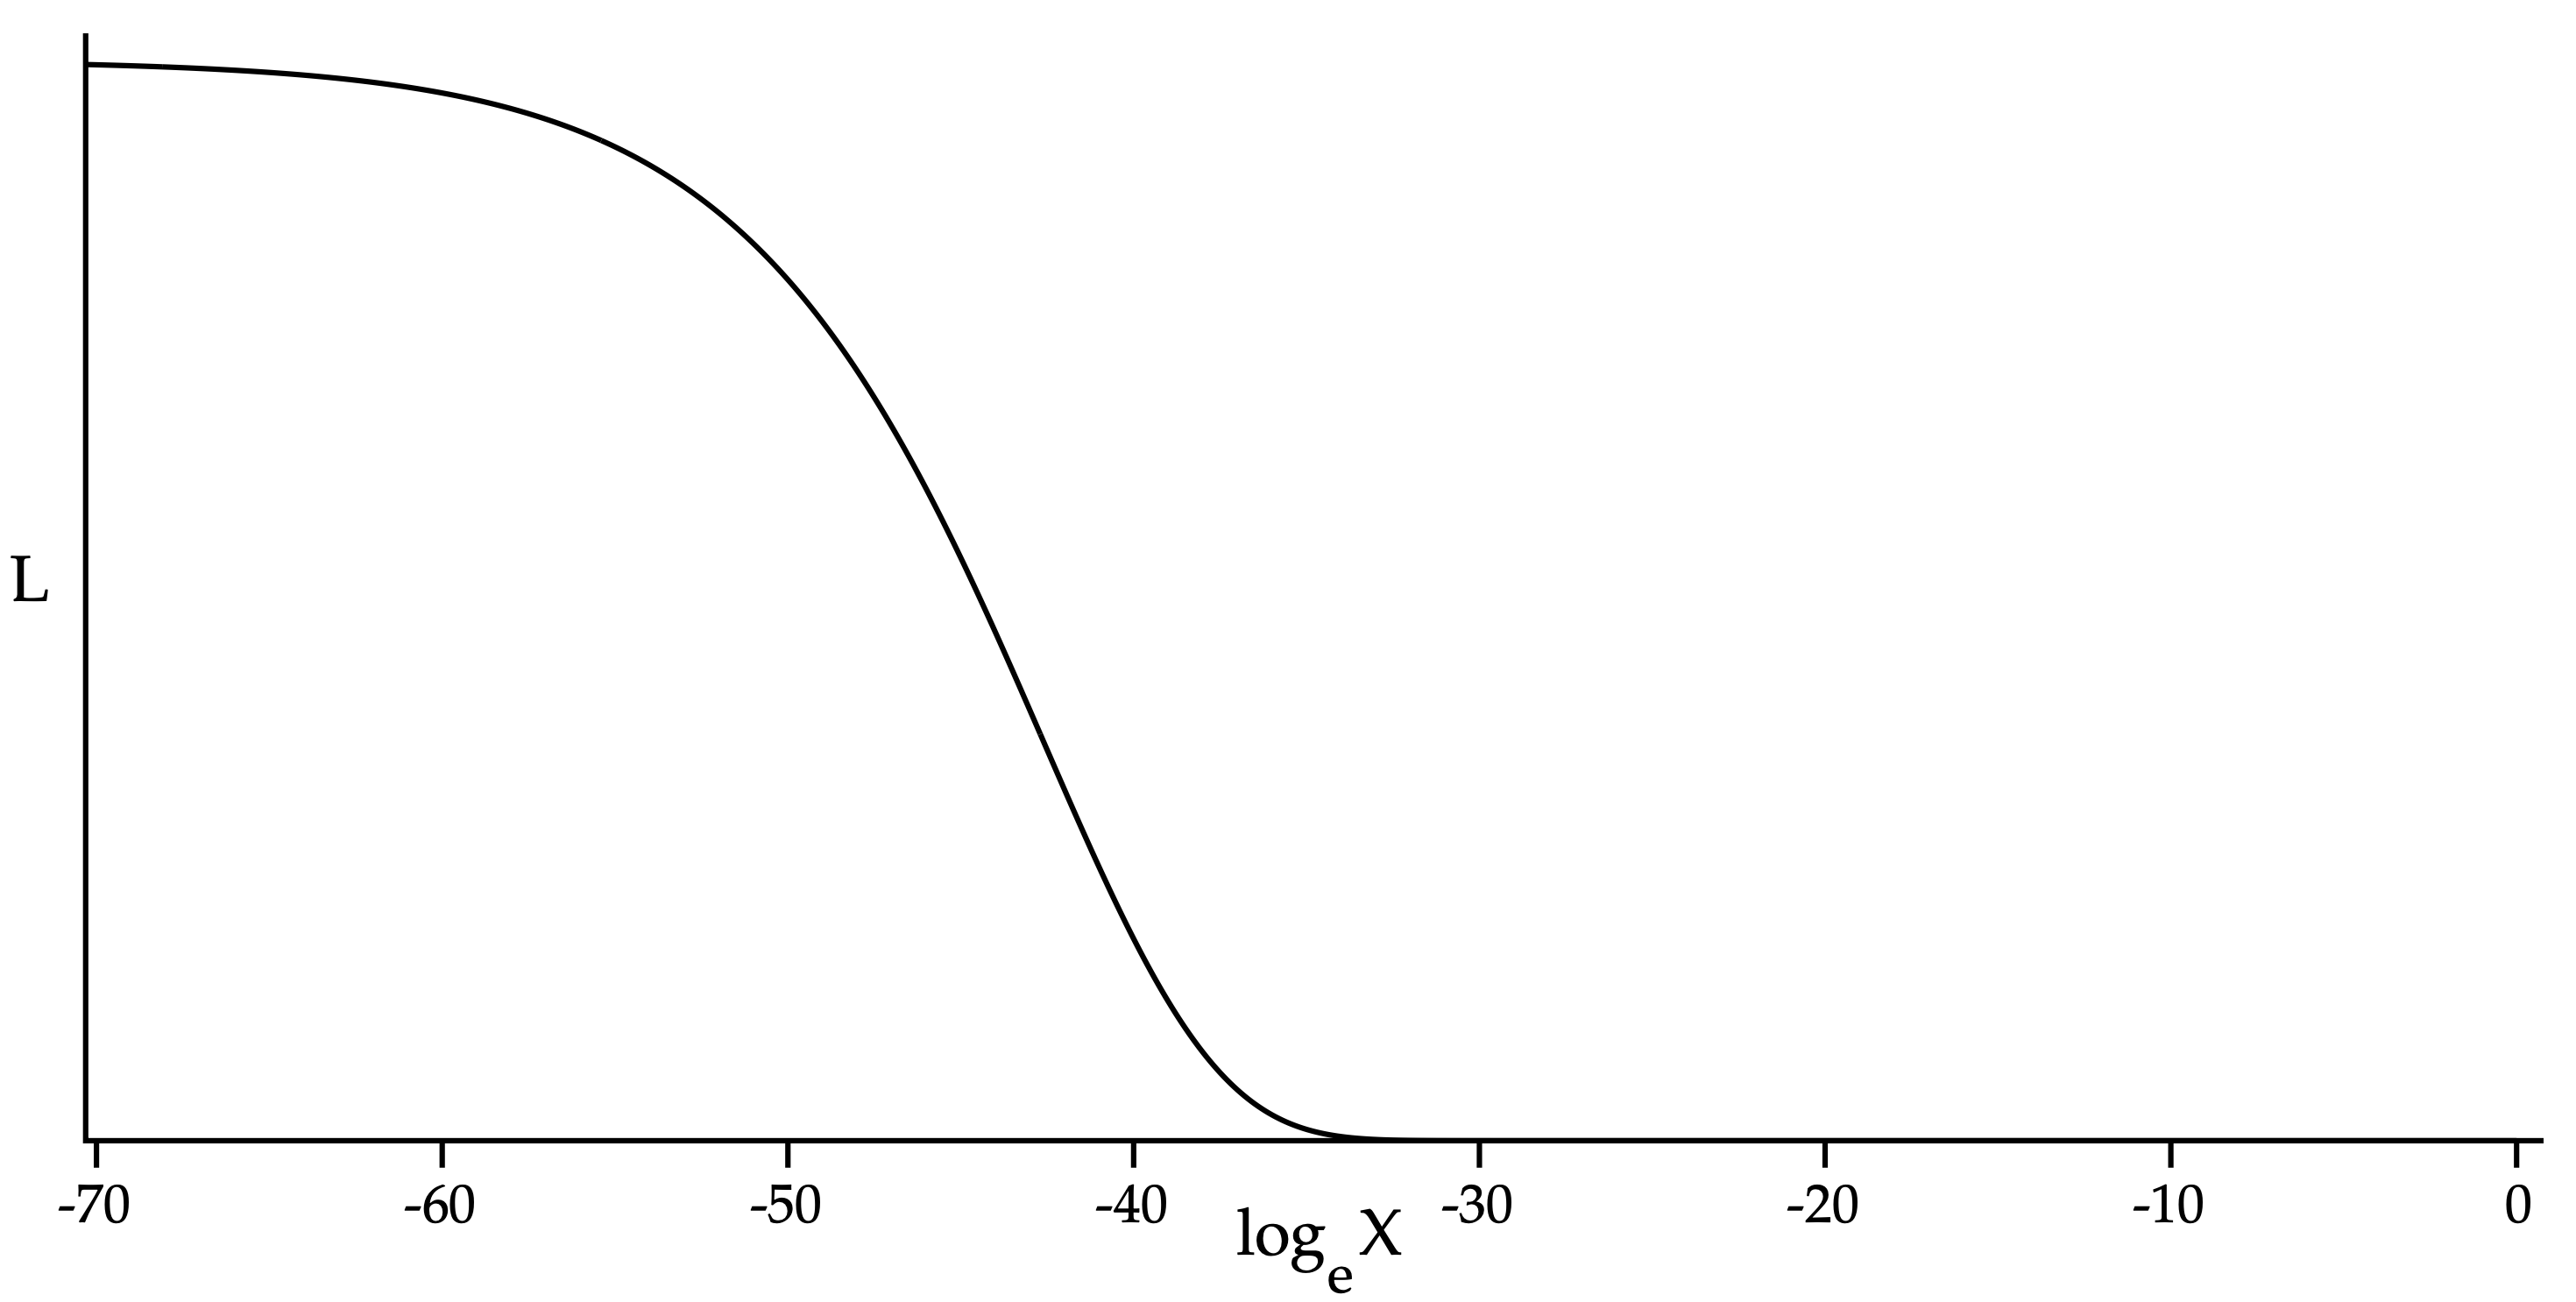
\includegraphics[width=1.0\textwidth]{Chapter2/Figs/Raster/Screenshot 2022-11-08 at 06.29.01.png}
\caption{ An example likelihood as a function of prior volume. Taken from \cite{10.1214/06-BA127}.}
\label{fig:skil1}
\end{figure}

Now let us try to gain an intuition by visually examining a nested sampling run in terms of its approximation of prior volumes. Let us first look at what an analytical plot of the likelihood as a function of prior volume may look like in \cref{fig:skil1} for some example likelihood.

\begin{figure} 
\centering    
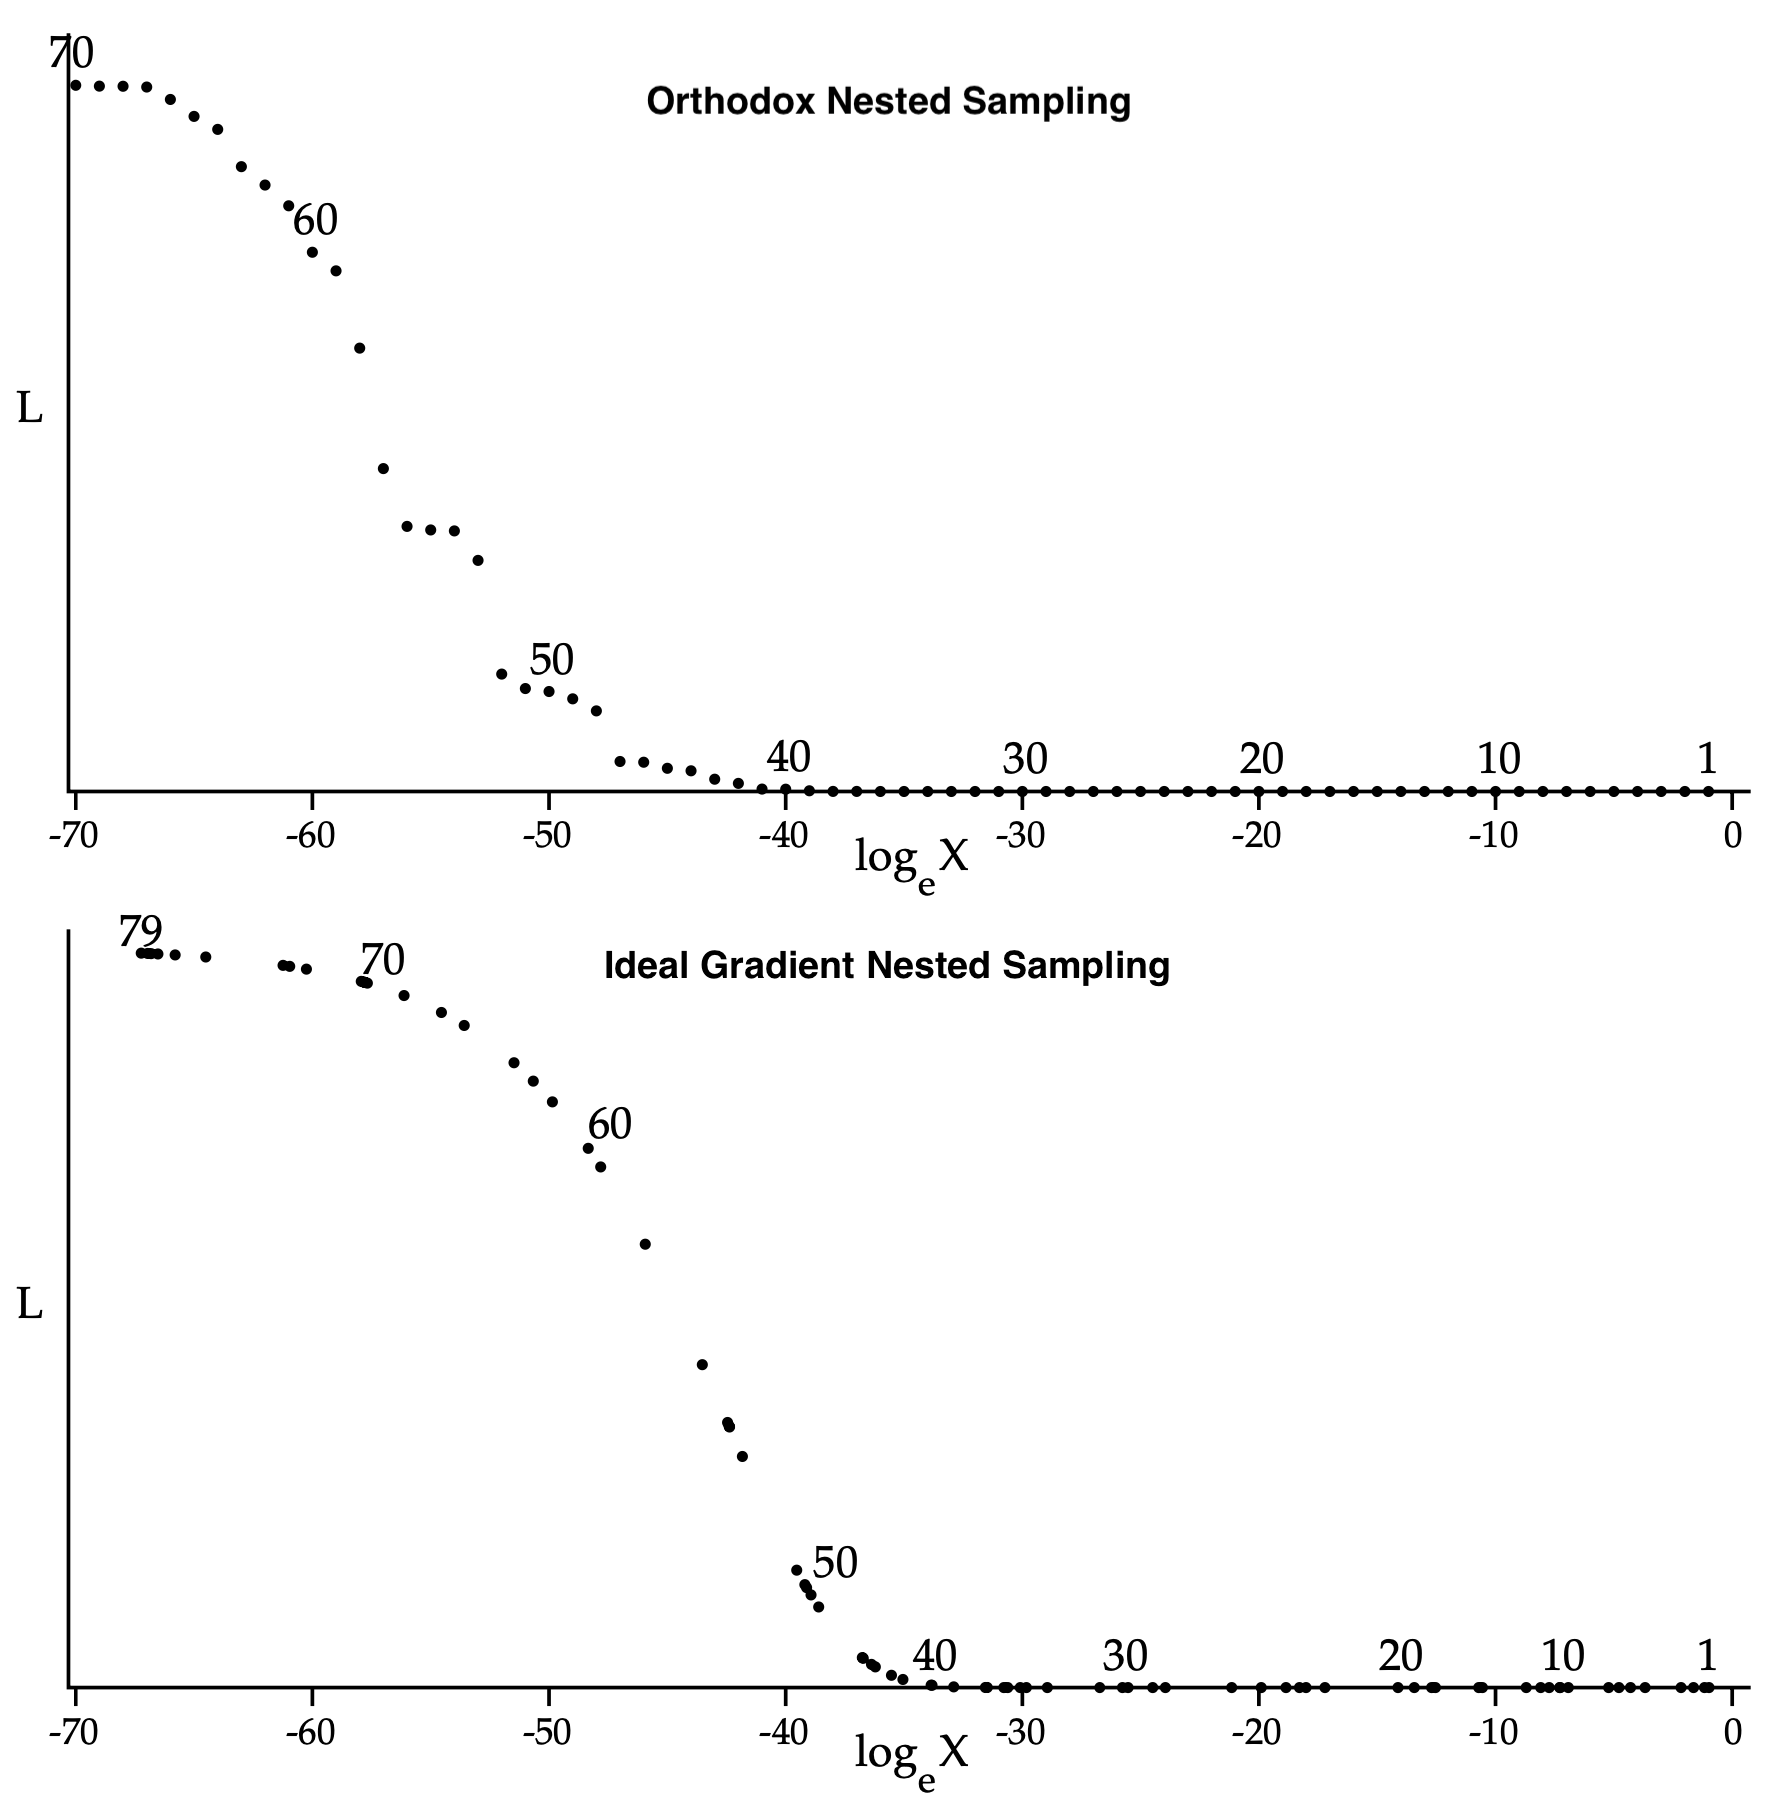
\includegraphics[width=1.0\textwidth]{Chapter2/Figs/Raster/Screenshot 2022-11-08 at 06.33.03.png}
\caption{ Orthodox nested sampling and ideal gradient nested sampling simulations of the likelihoods plotted against prior volumes. These are nested sampling runs for the same example likelihood function as in \cref{fig:skil1}. The lower plot shows what we hope to get from gradient nested sampling based on the fundamental idea of utilising a `prior on curves'. The numbers above the points denote the ordering of their respective likelihood magnitudes; for example, the point labelled by $50$ would have a likelihood which is higher than the $49$ previous poi§nts. The likelihood values of each respective point are known with zero associated error. Thus, the two plots only differ in terms of the $\log X$ locations of points--meaning that each point's respective likelihood is the same for both methods. The gradient nested sampling points have varying gaps in the x-axis meanwhile the orthodox nested sampling has constant gaps. This is because the orthodox method assumes a constant shrinkage of the prior volume regardless of the change in likelihood at each new sample, however gradient nested sampling uses this likelihood change as a guide to approximate the prior volume shrinkage. The reader should keep in mind that nested sampling calculates the Bayesian evidence through a sum containing prior volumes and their respective likelihoods. Thus, if we reduce the errors on the prior volume estimates, we reduce the carried error on the results of nested sampling. Altered from \cite{10.1214/06-BA127}.}
\label{fig:skil2}
\end{figure}

Let us now examine, for this example likelihood in \cref{fig:skil1}, the `orthodox nested sampling' results for the prior volumes estimates in comparison with the ideal gradient nested sampling prior volume estimates. Refer to \cref{fig:skil2} for a visualisation of this. The reader should keep in mind that in nested sampling the set of sampled likelihoods have no error associated with them. This means that the $y$-axes coordinates in the plots in \cref{fig:skil2} have no error associated with them and that the entirety of the error comes from the prior volumes, represented by the x-axes. Note that the points in the gradient nested sampling case in the figure more closely follow the true shape, as shown in \cref{fig:skil1}, of the likelihood function. This is because the error on the prior volumes is reduced in gradient nested sampling due to the usage of the information encoded within the gradient of the likelihood. The creator of nested sampling, John Skilling, was adamant that a `prior on curves' must exist but we just need to find it~\cite{paris2022}. Since gradient nested sampling allows us to more accurately simulate the prior volumes for known log-likelihood values, this results in a more accurate nested sampling run and thus more accurate Bayesian evidence calculations. Now that we have covered the motivation and general intuition behind gradient nested sampling, we can get into a rigorous derivation in the next section.




\section{\label{sec:level2}Theory}\label{sec:theorygrad}

The theoretical underpinning for gradient nested sampling is rooted in using the smoothness and continuity of the likelihood function to make a better estimate of the prior volume at each iteration. A priori this should be better than a completely random guess of prior volume that does not use any of the useful information encoded within the gradient of the likelihood being sampled. Current methods of determining prior volume return a set of $X_i$ that may well be used against any other likelihood to generate an evidence\footnote{As previously stated, the orthodox nested sampling algorithm is invariant under monotonic transformations of the likelihood function.} (given the same choice of dead and alive points of course). 

To begin with the gradient nested sampling derivation, we must examine a set of $k$ consecutive points in ${X_i}$ where the gradient,
\begin{equation}
g= \frac{d \log X}{d \log L},
\label{eq:ggg}
\end{equation}
%
is approximately constant. Using the equations 
%
\begin{align}
g \delta \log L_{i} = \delta \log X_i= -\log t_i, \\
P(\log t_{i})=Ne^{N \log t_i},
\label{eq:glogt}
\end{align}
%
where $N$ is the number of `live points'. We thus find
%
\begin{align}
P(\delta \log L_i|g)= gNe^{Ng \delta \log L_i},
\end{align}
%
where we substituted  $\log t_i= g\delta \log L_i$ and used 
\begin{equation}
    \frac{d \log t_i}{d\delta \log L_i}= g.
\end{equation}
For a given set of likelihood values $D= \{ \delta \log L_{i+1-(k/2)},\delta \log L_{i+2-(k/2)},...,\delta \log L_{i+(k/2)} \}$, which span $k$ consecutive points chosen in a deliberately symmetrical fashion around $i$, we have
%
\begin{align}
P(D|g)&= \prod_{j=i+1-(k/2)}^{i+(k/2)} P(\delta \log L_j|g) = \prod_{j=i+1-(k/2)}^{i+(k/2)} gN \exp (Ng \delta \log L_j).\\
&=  (gN)^k\exp\left(Ng \sum_{j=i+1-(k/2)}^{i+(k/2)}\delta \log L_j\right).\\
&=  (gN)^k\exp\left(Ng (\log L_{i-k/2} - \log L_{i-k/2})\right).
\end{align}
%
We find that $\log t_i$ follows a gamma distribution \cite{hogg_craig_1971} of the form:
%
\begin{equation}
P(\log t_i) \propto \frac{N^k}{\delta \log L_i}(\log t_i)^{k-1} \exp \left( \log t_i \frac{N(\log L_{i+k/2}-\log L_{i-k/2})}{\log L_i-\log L_{i-1}} \right).
\label{eq:blab}
\end{equation}
%
This is the main result of gradient nested sampling. \footnote{From this derivation we learn that we may use a function to draw samples from a gamma distribution, in our code to simulate our $\log t_i$ values for gradient nested sampling.} Note that for this step we used used Bayes' theorem with prior $\pi (g)=1/g$ to flip the conditional from $g$ to $D$. One must keep in mind that one could use other priors, $\pi(g)$, in this derivation. However our results, explored later in this chapter, that it might be the ideal prior given accurate information on the gradient of the likelihood and at the very least is superior to all other priors we tested. So as to not break the flow of this derivation we shall cover the different priors in more detail later in \cref{sec:exploring}. This step also used
%
\begin{equation}
  \frac{dg}{d\log t_i}  = 1/(\delta \log L_{i}),
\end{equation}
%
which is derived from \cref{eq:glogt} using that $\delta \log L_{i}$ is known and a constant. 

\begin{figure} 
\centering    
\includegraphics[width=1.0\textwidth]{Chapter2/Figs/Raster/regeneratedfig2_3.pdf}
\caption{ Plots showing the accuracy of gradient nested sampling over varying $k$-values. The $y$-axis represents the $\log Z$ value averaged over 100 different sets of $\log X$ simulations. That is, each point plotted is the average over 100 different nested sampling runs with the same set of $\log L$ samples but each with its own simulated $\log X$ set. Several different variations of gradient nested sampling are plotted and have been elaborated upon in the text.}
\label{fig:loglolol}
\end{figure}

Now that we have understood how to reach the main result, \cref{eq:blab}, it can further be used to give us the expectation value and standard deviation:
%
\begin{equation}
  E(\log t_i)=  \frac{k(\log L_i-\log L_{i-1})}{N(\log L_{i+k/2}-\log L_{i-k/2})}, 
\label{eq:mean}
\end{equation}
%
\begin{equation}
  \sigma(\log t_i)=  \frac{\sqrt{k}(\log L_i-\log L_{i-1})}{N(\log L_{i+k/2}-\log L_{i-k/2})}.  
\label{eq:err}
\end{equation}
%
This result is very suggestive. Orthodox nested sampling produces an error of 
%
\begin{equation}
    \sigma(\log t_i)= \frac{1}{\sqrt{N}}
\end{equation}
%
since it estimates the prior volumes using the less accurate power law distribution. However, from \cref{eq:err} we find that for gradient nested sampling we have
%
\begin{equation}
  \sigma(\log t_i) \sim O(\frac{1}{ \sqrt{Nk}}). 
\label{eq:gamm}
\end{equation}
%
This gamma distribution error is a factor of $\sqrt{k}$ smaller than the power law error in orthodox nested sampling. This means that the resulting prior volume values will be more accurate for gradient nested sampling using the proposed gamma distribution. Thus, theoretically, resulting in more accurate posterior samples and evidence calculated from gradient nested sampling as compared to orthodox nested sampling. 
The way we arrive at the result in \cref{eq:gamm} is noting that if as we assumed in our derivation above the gradient is constant over the $k$ points that span our data set, $D$, then the fraction from \cref{eq:err} above
%
\begin{equation}
\frac{(\log L_i-\log L_{i-1})}{(\log L_{i+k/2}-\log L_{i-k/2})}   \propto \frac{1}{k}. 
\end{equation}
%
This is because the distance between each of the $k$ points on the $\log L$ vs $\log X$ graphs should be the same if the gradient is constant and the numerator is the vertical-axis distance between two points that are 1 iteration away from each other and the denominator is the vertical-axis distance between two points that are $k$ iterations away from each other.




\section{Exploring Different data sets $D$ and Priors}\label{sec:exploring}
An astute reader may have noticed a subtlety in the derivation: the initial and final $k/2$ `dead points' are orphan terms for which we would not be able to follow this same process of gradient nested sampling. The reason being that the above derivation assumes there exist $k/2$ points before and after the point we are trying to simulate using the gamma distribution. However, to avoid this issue, the first and last $k/2$ points can be assumed to follow the usual power law distribution. We can do this because $k$ is a small number in comparison with the total dead points and thus the change in total posterior mass in the final calculation would be negligible. 

Another subtlety is that this result assumes that $k$ is even. This is, however, not necessary and the breaking of generality stems from how we chose the set of consecutive points $D= \{ \delta \log L_{i+1-(k/2)},\delta \log L_{i+2-(k/2)},...,\delta \log L_{i+(k/2)} \}$. The reason for the symmetrical nature of these points about $i$ is that the crux of the calculation is trying to find the average of the gradient for our log-likelihood over the $k$ points in $D$. Then, we use this estimated average gradient to approximate how much our $\log X$ should have changed given that we have a known change in $\log L$. It is analogous to the case of a two dimensional curve, $y=f(x)$, for which we approximate the gradient by drawing a tangent and using the known change in the $y$-coordinate, we guess the change in $x$-coordinate. Given this information in the example, we accordingly use it to guide our estimate of the corresponding change in the horizontal axis coordinate. Thus, for defining $D$ we would like to use a string of points that best approximate the gradient at point $i$. Intuitively, this would be best performed through a set of points chosen symmetrically about $i$. There are different ways to select sets of points symmetrically about $i$ even allowing for odd $k$. However, that would make the derivation in \cref{sec:level2} more difficult to follow. The way it has been laid out in this derivation is how it is easily digested while still being symmetrical. This is since that the final result has that the $k$ we used to label our data points in $D$ is exactly the same as the $k$ in the resulting gamma distribution, $\Gamma (k,\theta)$, that is followed by the $\log t_i$. For completeness we define the gamma distribution: if a random variable follows the gamma distribution $X \sim \Gamma (k,\theta)$ then we have the probability density function for $X= x$ as:
%
\begin{equation}
    f(x;k,\theta) = \frac{x^{k-1} \exp (-x/\theta)}{\theta^k \Gamma(k)}, 
\end{equation}
%
where $\Gamma(k)$ is the gamma function evaluated at $k$.

Our particular choice of the prior, $\pi (g)=1/g$, also leads to this compact result mentioned in the line above. Though we initially made these choices for aesthetic reasons and neatness, it turns out that no other prior that we test gives as accurate results as this one.  In terms of the final results, changing the prior only changes the $k$ parameter that we input in the gamma distribution, $\Gamma ($k$,\theta)$, that generates the prior volumes. To avoid ambiguity, for now let us write the first parameter in the gamma distribution as an upper case $K$, $\Gamma ($K$,\theta)$. Using this terminology, our previous derivation arrived at $K=k$. However, if we used the one of the following priors, $\pi (g)$, instead: $\pi (g)=1$, $\pi (g)=1/g^2$, $\pi (g)=g$, we would get $K=k+1$, $K=k-1$, and $K=k+2$ correspondingly. We plot analyses of these other priors in \cref{fig:loglolol}. We shall also find that small shifts in the sequence of our $k$ points or changes from odd $k$ to even $k$ make immeasurable difference. In this chapter, we explore all plausible options to a realistic level. This includes the most symmetrical  with $2k+1$ points in $D$, with $k$ points ahead and behind $i$--this is plotted in \cref{fig:loglolol} as well.



\section{Results and Data} \label{sec:resdat}

\subsection{Initial Results}

Let us start by plotting the prior volumes themselves, as generated from the gamma distribution under our newly proposed gradient nested sampling scheme. It must be emphasised that for any one particular figure in this section we shall only use one set of $\log L$ samples, to generate different full sets of corresponding $\log X$s. A nested sampling run requires a set of sampled $\log L$ and a correspondingly generated set of $\log X$. Since the prior volumes are generated probabilistically, one set of sampled log-likelihoods can be used to generate many sets of $\log X$s. This is due to the computational restrictions regarding generation of a set of likelihood samples from large data sets for a nested sampling run. For example, the Gaia Data Release 2 is comprised of $340$ billion measurements of celestial sources~\cite{gaia_in_the_uk}. Generating just one set of $\log L$s for nested sampling takes weeks of compute time in the context of cosmology. So, one can always assume throughout this chapter that all separate sets of $\log X$s in the multiple nested sampling runs within a singular figure correspond to just one set of $\log L$s. 

Throughout our results in this chapter we shall use a toy model log-likelihood taken from ref \cite{10.1214/06-BA127}. This allows us to have precise and analytical values for $\log L$, $\log X$ and $\log Z$ to compare to the results of our proposed method. The toy model log-likelihood is

\begin{equation}
    \log L(\log X) = -\frac{\exp (\frac{2\log X}{C}) }{2 \sigma^2},
\label{eq:toy}
\end{equation}
%
with a flat prior 
%
\begin{equation}
    \mathrm{prior}(\theta) = \frac{(C/2)!}{\pi^{C/2}}
\end{equation}
%
and log evidence being 
%
\begin{equation}
   \log Z = \log( (C/2)!) + \frac{C}{2}\log ((2\sigma^2)).
\end{equation}
%
Note that we denoted the prior by $\mathrm{prior}(\theta)$, so as to not have it confused with the prior on the gradient, $\pi(g)$. Also the fact that the right-hand side does not depend on the parameters, $\theta$, is due to it being constant for all parameter values--the definition of a flat prior.We take $C=10$ and $\sigma = 0.01$ for all the following results.

Now we have a picture of the likelihood and the prior that we shall use to run tests for gradient nested sampling. So let us then plot the preliminary results of the prior volumes as generated by the gradient nested sampling scheme in \cref{fig:logX1}.
%

\begin{figure} 
\centering    
\includegraphics[width=1.0\textwidth]{Chapter2/Figs/Raster/regeneratedfig2_5.pdf}
\caption{ The plots of the toy model log-likelihood from \cref{eq:toy}, and its derivative (this is the inverse of $g$ from \cref{sec:theorygrad}), as a function of log X. The plot also demonstrates that in the direction of increasing iteration number, $i$, of the nested sampling algorithm the $\log X$ value decreases. This is knowledge is pertinent in understanding the subtleties of the algorithm.}
\label{fig:expo}
\end{figure}


\begin{figure} 
\centering    
\includegraphics[width=1.0\textwidth]{Chap2_fig1}
\caption{This figure contains 10 simulated sets of $\log X$s plotted for each simulation method. Each separate line represents a separate $\log X$ simulation which could be used for a separate nested sampling run. Again, all $50$ $\log X$ sets in this figure correspond to the same singular set of log-likelihood samples. The number of live points used was $1000$, and the number of dead points by the end was $100,000$. The $y$-axis represents how far the $\log X$ simulation has deviated from the `real' $\log X$ that has been calculated analytically. The black horizontal line corresponds to the ideal $\log X$ run. The orange lines labelled `power law distributed' refers to the usual method for simulating $\log X$s. The other lines are generated, using the method we describe in the text, with varying $k$ parameter values.}
\label{fig:logX1}
\end{figure}

\cref{fig:logX1} visualises multiple sets of simulated prior volumes for multiple nested sampling runs and how they scatter from the true prior volume. It shows how gradient nested sampling reduces the errors on the prior volume simulations as compared to orthodox nested sampling. The closer a simulated $\log X$ set is to the true $\log X$ set in \cref{fig:logX1}, the lesser it would deviate from the zero. Thus, since the power-law lines scatter furthest from the centre line, they seem to have the least precision. Examine the brown lines, where we used our proposed gamma distribution method to generate the $\log X$s with $k$ equal to the number of live points. These brown lines have the largest precision but least accuracy--meaning if one averages all the brown $\log X$s, it would average to a completely biased answer. Increasing the $k$ parameter results in a trade-off between accuracy vs precision. When we increase the precision by increasing the $k$ value, it is a trade-off with accuracy. If the $k$-value is too high, the `estimated' gradient (from \cref{eq:est}) starts to become smaller than the actual gradient. This is because of the exponential relation between $\log L$ and $\log X$. It is such that, as the number of iterations of nested sampling increases the gradient decreases. This is visualised in \cref{fig:expo}, the gradient of $\log L$ vs $\log X$ decreases as the iterations of nested sampling increase--one must keep in mind that $\log X$ becomes more negative as the iterations increase, so think of going from right to left in the \cref{fig:expo} as we increase the iterations. In other words, as the iteration number, $i$, increases the flatter the graph between $\log L$ and $\log X$ becomes. This simply means that if we choose a large enough $k$, the tangent that we draw to approximate the gradient at point $i$ becomes less and less accurate for estimating the real gradient. Thus one sees that the red, purple and brown lines skew upwards. This is because the estimated gradient is smaller than it should be and thus the algorithm thinks that for a given $\log L$ increase, the $\log X$ decrease should have been less than it is. Again, this is due to the biased `estimated' gradient that is smaller than it should be in the direction of increasing iteration number (or decreasing $\log X$). So it adjusts the $\log X$ in a biased way, which is larger than the actual analytical value. This is why, in \cref{fig:logX1}, the increasing $k$ values result in more positive values for $(\log X -\log X_{\mathrm{Analytical}})$. To better understand this line of geometric reasoning one should carefully examine \cref{fig:expo} keeping in mind $\log X$ decreases as iteration number, $i$, increases.



The discussion in the paragraph above was useful to gain a sense of intuition as to how particular curvatures and gradients of the likelihood function may interfere with gradient nested sampling. However, the conclusion, which would be more generally applicable for all likelihoods, is that it does not matter how large the second derivative of the log-likelihood function is so long as $k$ is small enough relative to the number of live points.


The conclusion that we can draw from our preliminary results in \cref{fig:logX1} is that the $k$=10 value is seemingly the best trade-off between precision and accuracy. So let us start off by further analysing this before exploring other variations.


\begin{figure} 
\centering    
\includegraphics[width=1.0\textwidth]{Chapter2/Figs/Raster/chap2_fig3.pdf}
\caption{ A comparison of the $\log Z$ histogram plots as produced by the orthodox nested sampling algorithm and our newly proposed gradient nested sampling. The black vertical line represents the true analytical value of $\log Z$. The number of live points used throughout were $1000$.}
\label{fig:loll}
\end{figure}

\cref{fig:loll} is a histogram plot of the log-evidences produced by gradient and orthodox nested sampling runs. We can see from \cref{fig:loll} that gradient nested sampling did not produce our expected result. The expected result was gradient nested sampling producing log-evidence histogram plots with the peak shifted closer to the true $\log Z$ value. Orthodox nested sampling produces an estimate of the evidence to within its error margins. Gradient nested sampling produces an apparently more accurate evidence value, but with an overconfident error bar which does not encompass the true value.

It does not seem that the issue would be fixed by the implementation of `dynamic nested sampling'~\cite{Higson_2018} but, since it has become an industry-standard, we still coded a dynamic gradient nested sampling version. Dynamic nested sampling is another version of nested sampling in which the number of live points is variable with each nested sampling iteration, instead of the live points being constant throughout the whole process.

We shall briefly go over the formulae used in the dynamic gradient nested sampling at this point. Note that the crucial difference in this definition will be the dependence of $N_i$ on the iteration number, as the number of live points now change for every nested sampling iteration. Examine a set of $k$ consecutive points in ${X_i}$ where the gradient,
\begin{equation}
g= \frac{d \log X}{d \log L},
\end{equation}
%
is approximately constant. Using the equations 
%
\begin{align}
g \delta \log L_{i} = \delta \log X_i= -\log t_i, \\
P(\log t_{i})=N_i e^{N_i \log t_i},
\end{align}
%
where $N_i$ is the number of `dynamic live points' at iteration number, $i$. We then find
%
\begin{align}
P(\delta \log L_i|g)= gN_ie^{N_i g \delta \log L_i},
\end{align}
%
where we substituted  $\log t_i= g\delta \log L_i$ and used 
%
\begin{equation}
    \frac{d \log t_i}{d\delta \log L_i}= g.
\end{equation}
%
For a given set of data points $D= \{ \delta \log L_{i+1-(k/2)},\delta \log L_{i+2-(k/2)},...,\delta \log L_{i+(k/2)} \}$, which spans $k$ consecutive points chosen in a deliberately symmetrical fashion around $i$, we have
%
\begin{align}
P(D|g)&= \prod_{j=i+1-(k/2)}^{i+(k/2)} P(\delta \log L_j|g) = \prod_{j=i+1-(k/2)}^{i+(k/2)} gN_j\exp({N_jg \delta \log L_j}).\\
&\propto  g\exp\left( g \sum_{j=i+1-(k/2)}^{i+(k/2)} N_j \delta \log L_j\right).
\end{align}
%\left( \prod_{j=i+1-(k/2)}^{i+(k/2)}(gN_j)^k\right) 
Note that this time we vary the number of live points at each iteration and thus we could not take it out of the sum. Then we get that $\log t_i$ is follows a gamma distribution \cite{hogg_craig_1971} of the form:
%
\begin{equation}
P(\log t_i) \propto \frac{(\log t_i)^{k-1} }{\delta \log L_i}\exp \left( \log t_i \frac{\sum_{j=i+1-(k/2)}^{i+(k/2)} N_i \delta \log L_j}{\log L_i-\log L_{i-1}}\right).
\label{eq:uiui}
\end{equation}
%
Here, we used used Bayes' theorem with prior $\pi (g)=1/g$ to flip the conditional from $g$ to $D$. This step also used
%
\begin{equation}
  \frac{dg}{d\log t_i}  = 1/(\delta \log L_{i}),
\end{equation}
%
which is derived from \cref{eq:glogt} using that $\delta \log L_{i}$ is known and a constant. Utilising the result from \cref{eq:uiui}, we use a gamma distribution sampling function in the dynamic gradient nested sampling code to simulate $\log t_i$s. It is tested out as seen in \cref{fig:logL function}, where we plot the log-evidence values produced by dynamic orthodox and dynamic gradient nested sampling--that is, with variable number of live points. As we thought, it still does not do what we expect from gradient nested sampling.

\begin{figure} 
\centering    
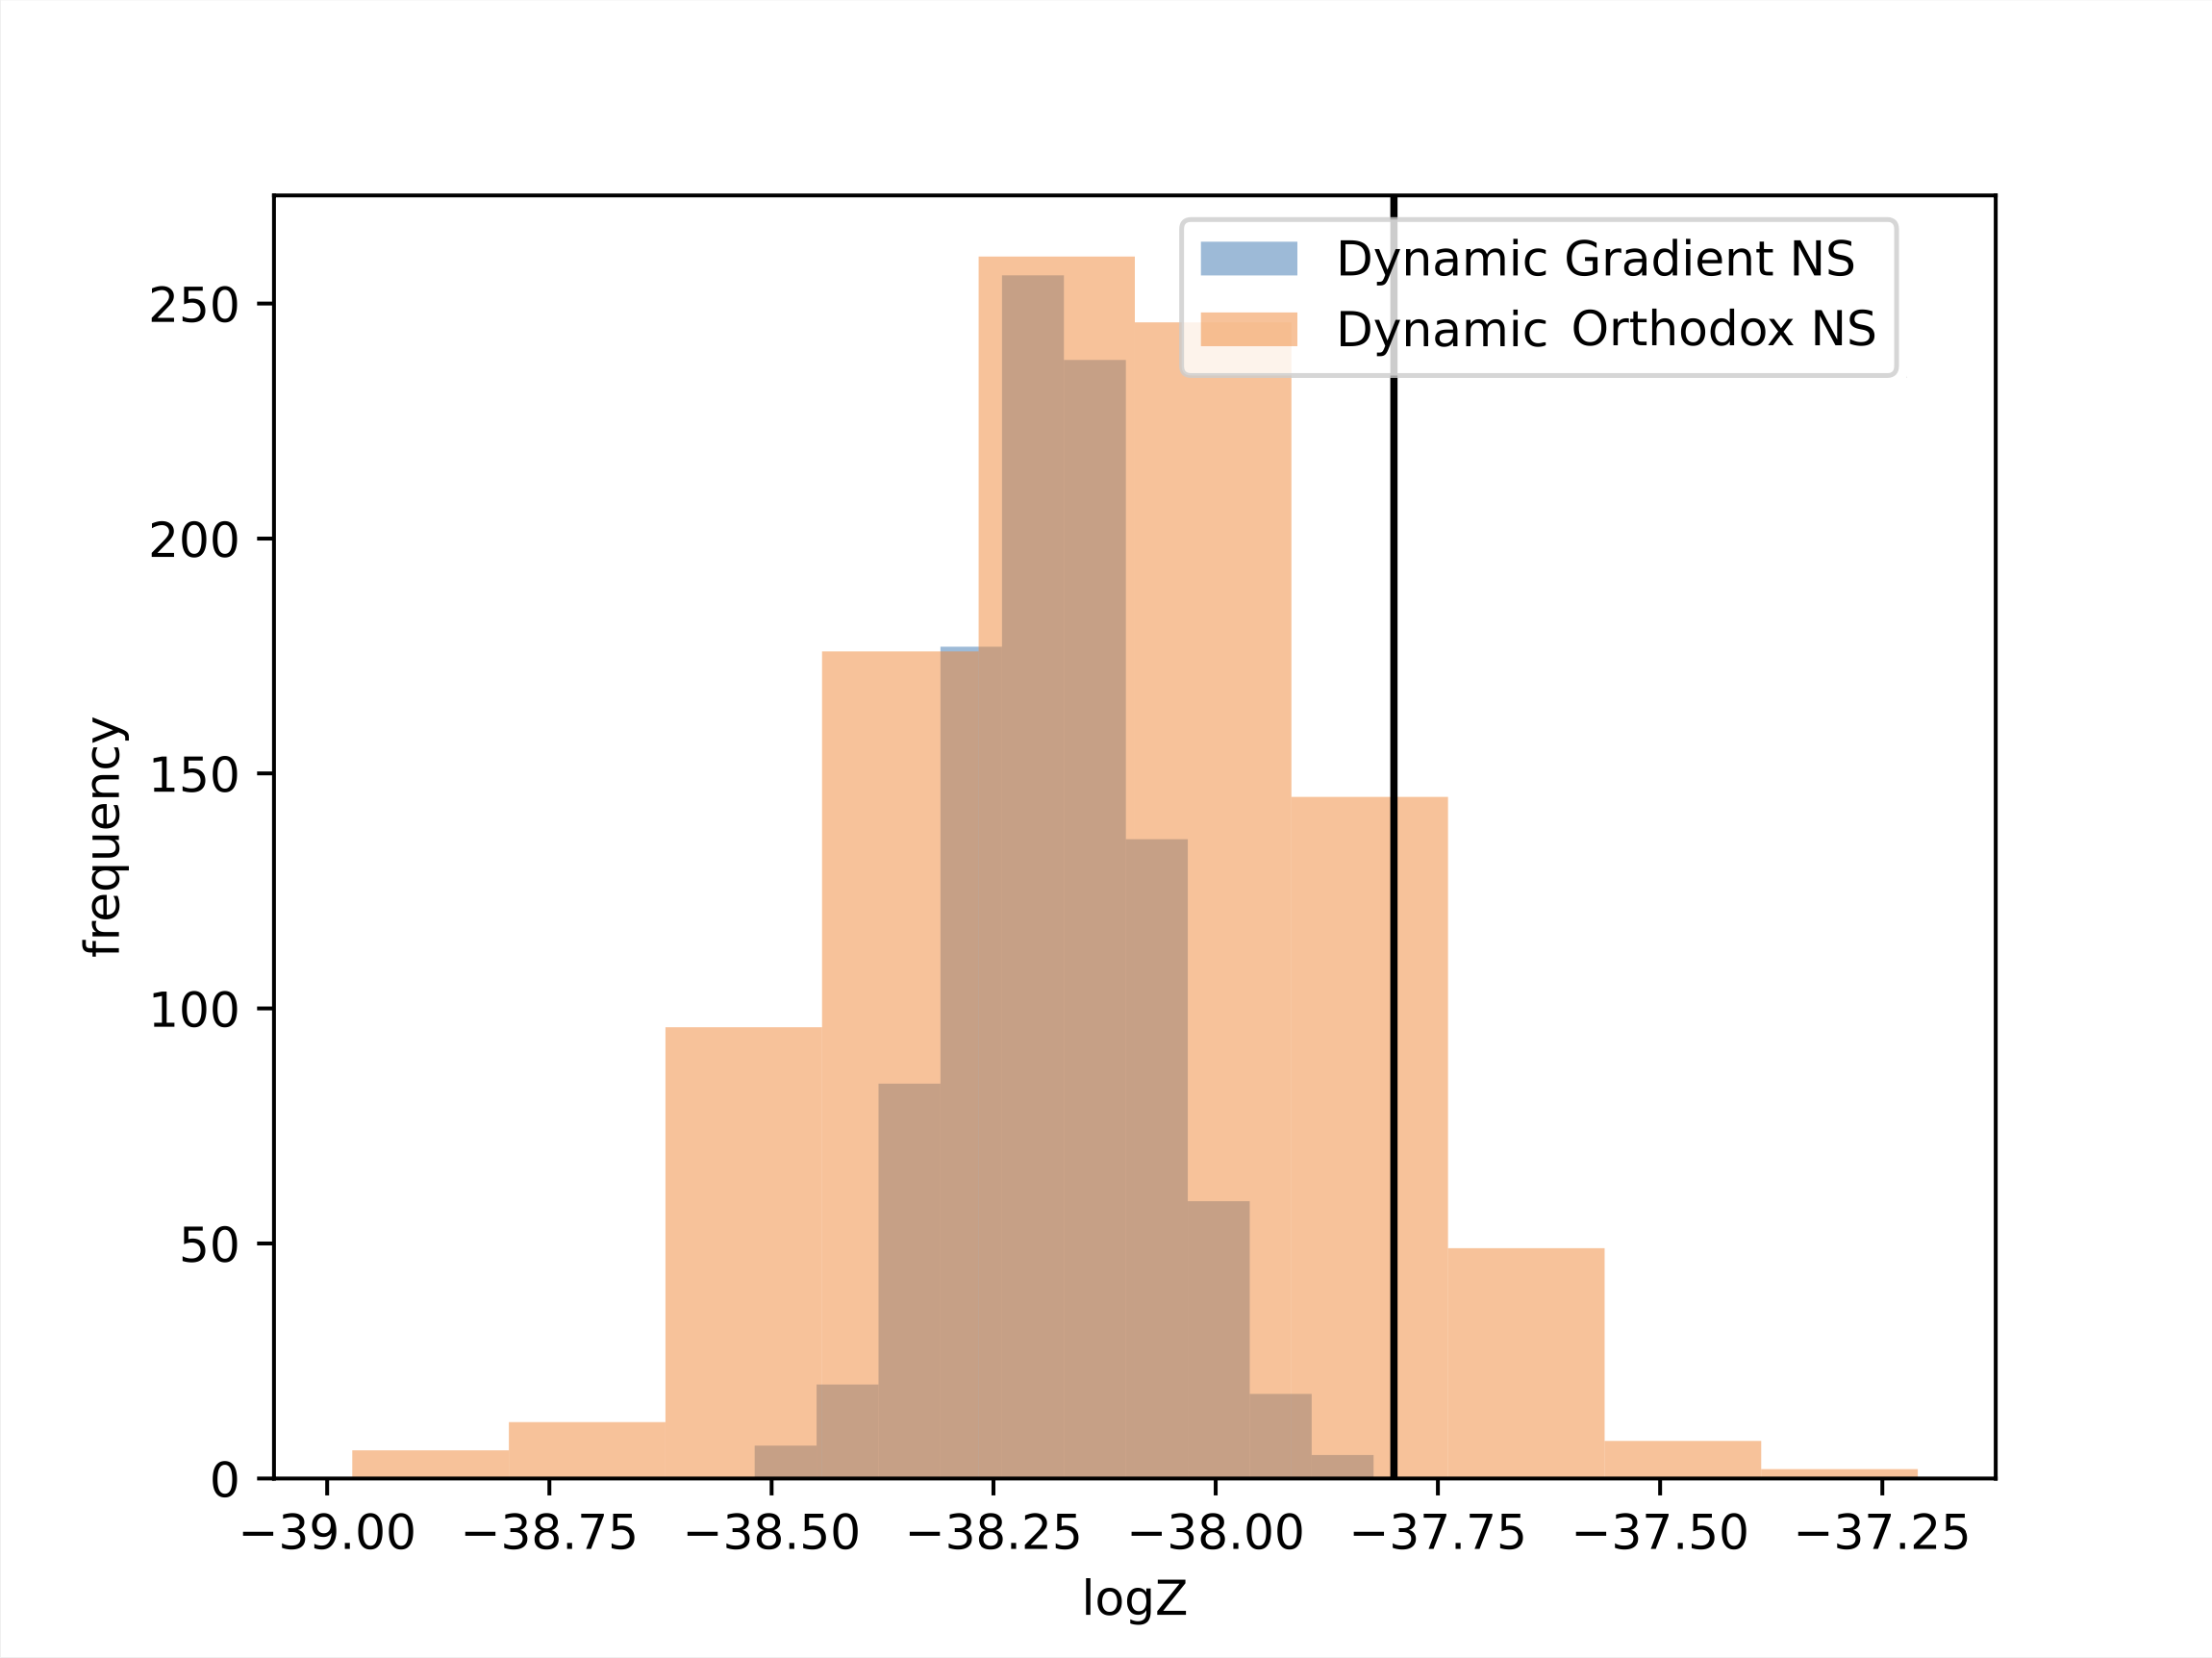
\includegraphics[width=1.0\textwidth]{Chapter2/Figs/Raster/Screenshot 2023-01-03 at 17.40.14.png}
\caption{A comparison of the $\log Z$ histogram plots of the orthodox nested sampling algorithm (orange histogram) and our newly proposed gradient nested sampling (blue histogram) both now with a dynamic number of live points~\cite{Higson_2018}. This is a similar plot to \cref{fig:loll} with the only difference being a dynamic number of live points. The black vertical line represents the true analytical value of $\log Z$. We initiate each nested sampling run with $5000$ live points and incrementally go down to $100$, subtracting one live point at each subsequent iteration.}
\label{fig:logL function} 
\end{figure}




\begin{figure} 
\centering    
\includegraphics[width=1.0\textwidth]{Chapter2/Figs/Raster/regeneratedfig2_8.pdf}
\caption{Graphs showing the accuracy of our proposed gradient nested sampling method over varying $k$ values. The $y$-axis represents the $\log Z$ value averaged over 100 different sets of $\log X$ simulations. That is, each point plotted is the average over $100$ different nested sampling runs with the same set of $\log L$ samples but each with its own simulated $\log X$ set. These $100$ different nested sampling runs also allow us to calculate the variance for the error bars that can be seen on the lines. The blue line shows the values calculated using the estimated gradient, and the red line shows the values calculated using the analytical gradient. The red line used the analytical $\theta$ from \cref{eq:t2}--for a practical implementation this would not be possible, it is only for the toy model that we have the privilege of the analytical expression. The blue $k$=0 point represents the average of $100$ log-evidence values generated from the orthodox nested sampling algorithm. The true $\log Z$ value is plotted as the black horizontal line.}
\label{fig:loglol}
\end{figure}

The issue we are met with again is the determining of an ideal $k$ value. The $k$ value alone does not mean much. The same $k$ can produce vastly different results depending on the number of live points used during the run. From this point onward  we shall stick to non-dynamic nested sampling with $1000$ live points for every orthodox nested sampling and gradient nested sampling run. This is to reduce the number of variables within the hyperparameters of nested sampling algorithm itself. Especially since we did not find any utility in dynamic nested sampling regardless. In an effort towards the optimisation of the $k$ parameter we plot graphs in the next subsection with varying values of $k$, and we also compare these results to `analytical' gradient nested sampling. Where `analytical' gradient nested sampling is a version that uses the fact that our toy likelihood allows us to have an exact expression relating likelihood to prior volumes--which wouldn't be the case for cosmology applications. 


\subsection{Analytical Gradient Nested Sampling for Comparison in Context of Toy Problem}




\cref{fig:loglol} shows that varying the $k$ value is, essentially, not making any useful difference. One may think that \cref{fig:logX1} suggests otherwise but increasing $k$ only reduces the spread of the prior volumes and makes them converge towards the same mean value as the orthodox nested sampling prior volumes--rather than converging it towards the true prior volume value. How this translates to graph \cref{fig:loglol} is that increasing $k$ only reduces the size of the error bars rather than actually bringing the evidence closer to the real value. The ups and downs of the blue graph in \cref{fig:loglol} are a product of nothing but the usual nested sampling stochasticity. One can note from these results that increasing $k$ only reduces the spread. This may seem beneficial at first glance but it is not because the error bars should intersect with the true $\log Z$ value represented by the black horizontal line. The optimistic conclusion in this figure is that if we use the analytical gradient our idea of `gradient nested sampling' works exactly as envisioned (examine the red line). This supports that the method is perhaps theoretically sound, but we need to find a way to reduce the error on the estimated gradient. The log evidence in the `analytical gradient' red line shifts closer to the true value and also has a smaller spread--but not smaller to the extent that it does not intersect with the true value.


For completeness' sake must shortly go over how analytical gradient nested sampling is run. From the derivation in \cref{sec:level2}, we learn that we may use a function to draw values from a gamma distribution in our code to simulate our $\log t_i$s. Where the $\theta$ parameter in $\Gamma (k,\theta)$ is 
%
\begin{equation}
   \theta = \frac{(\log L_i-\log L_{i-1})}{(\log L_{i+k/2}-\log L_{i-k/2})}.
\label{eq:t1}
\end{equation}
%
Gradient nested sampling in its form introduced in the `Theory' section 2.1 does not produce the required results, so we use the analytical version of this expression in the plots in \cref{fig:loglol} to find avenues of improvement. The analytical version is:
%
\begin{equation}
   \theta = \frac{(\log L_i-\log L_{i-1})g_i}{k}.
\label{eq:t2}
\end{equation}
%
This equation has a $g_i$ term in it, this is the same term from \cref{eq:ggg}. In the toy example we use in this paper (refer to \cref{sec:exploring}), $g_i$ is just the analytical gradient at point $i$ given by:

\begin{equation}
    g_i = -\exp(\frac{-2 \log X_i}{C})C \sigma^2.
\label{eq:nest}
\end{equation}


Here, $\log X_i$ is also the true analytical $\log X$ value at point with $\log L_i$, as calculated by our analytical expression given in \cref{eq:toy}. The estimated version of it is 

\begin{equation}
   g_{\mathrm{estimate}}= \frac{k}{(\log L_{i+k/2}-\log L_{i-k/2})}.
\label{eq:est}
\end{equation}


This is the version of $g$ that we would usually use in non-toy example implementations of gradient nested sampling. This is because we would not generally have the luxury of knowing the analytical value as we do for the toy example. 


To make sure the decisions we made during our derivation were not detrimental we plot \cref{fig:loglolol}. We try the different priors that we mentioned in \cref{sec:exploring}. We also try utilising a set of consecutive points $D$ such that it is completely symmetrical around $i$ (denoted by the blue plot in \cref{fig:loglolol})--$D= \{ \delta \log L_{i+1-k},\delta \log L_{i+2-k},...,\delta \log L_{i+k} \}$. This has $K=2k+1$ for the gamma distribution generating the $\log t \sim \Gamma(K,\theta)$. We also try the same again but excluding the $i$th point in $D$ and thus excluding from our gradient estimation (denoted by grey plot). The idea was that if there is some anomaly in the increment taken by point $i$ from its previous step, then we do not want to take this anomalous point into consideration for our correction calculations. In other words, we cannot correct the anomaly in term $i$ by using the gradient information from the $i$ term itself. We thus remove the $\log L_i$ point from $D$. This has $K=2k$ for $\log t \sim \Gamma(K,\theta)$. However, we find that from our results plotted in \cref{fig:loglolol}, that seemingly none of these ideas hold any merit. Additionally, it was already evident that the prior was not at fault, since referring to \cref{fig:loglol}, we observed the ideal results using the original prior and analytical gradient (refer to the red plot).


\begin{figure} 
\centering    
\includegraphics[width=1.0\textwidth]{Chapter2/Figs/Raster/regeneratedfig2_9.pdf}
\caption{ The gradients, $g$, plotted as a function of $\log X$. The green line is the plot of \cref{eq:est} and the red is a plot of \cref{eq:nest}. The blue plot is a rolling average of the green plot over the $k/2$ terms ahead and $k/2$ terms behind the point being plotted. In other words, the blue plot is a rolling average of the gradient of the $k+1$ points in the vicinity of the point being plotted.}

\label{fig:fffff}
\end{figure}

\begin{figure} 
\centering    
\includegraphics[width=1.0\textwidth]{Chapter2/Figs/Raster/regeneratedfig2_10.pdf}
\caption{ Plots which show the accuracy of gradient nested sampling over varying $k$ values. The $y$-axis represents the $\log Z$ values averaged over 100 different sets of $\log X$ simulations. That is, each point plotted is the average over 100 different nested sampling runs with the same set of $\log L$ samples but each with its own simulated $\log X$ set. The green line is the plot of the gradient nested sampling run utilising the estimated gradient expression (Eq. \ref{eq:est}) and the red is the plot of the gradient nested sampling run utilising the analytical gradient expression (Eq. \ref{eq:nest}). The blue line is a gradient nested sampling run which uses a rolling average of the gradient in place of the gradient in \cref{eq:est}. The rolling average is caried over the $3k$ terms ahead and $3k$ terms behind the point being plotted. For comparison, the $k$ value $=0$ point represents the results from the orthodox nested sampling algorithm.}

\label{fig:rrr}
\end{figure}

The results up until this point suggest that the main effort going ahead should be in finding better, more accurate estimators of the gradient $g$ (Eq. \ref{eq:est}). We plot $g$ as a function of $\log X$ in \cref{fig:fffff}. We see that the estimated gradient oscillated around the true gradient in a noisy, stochastic manner. The logical next step is to compute a rolling average of the estimated gradient and use it in place of the estimated gradient. We use these in the gradient nested sampling runs in \cref{fig:rrr}.





It seems that the rolling average of the gradient has finally reduced the noisiness enough to allow gradient nested sampling to work. This is quite an exciting result as it suggests we have a definite improvement to the precision and accuracy of nested sampling. We used a larger range of points in the rolling average for \cref{fig:rrr}, the rolling average was ran over $6k+1$ number of points. Of course, this number changes as $k$ changes. This rolling average range already becomes larger than the number of live points at $k=200$. We expect the gradient estimations to break down at the scale of the tangent being connected at points that are as far away as the number of live points, and this is exactly what we observe in our results. We increased the rolling average range because we noticed in \cref{fig:fffff} that $k+1$ points rolling averaged over is not enough to smooth out the noise. This starts to work extremely well around the $k=100$ mark, getting an almost perfect result at $k=150$ and then of course getting extremely biased again as $k$ reaches close to the number of live points. We previously established that this is roughly the order of $k$ at which gradient nested sampling starts to break down. 


\section{Conclusion}

Given the centrality of model comparison in science, and the fact that nested sampling represents the state of the art in numerically computing Bayes’ factors, any fundamental improvements in nested sampling accuracy would be deemed monumental. Our results show promise in this regard but they are still preliminary. Further work and scrutiny must be carried out in relation to gradient nested sampling. We concede that the rolling average method is a primitive way of getting gradient nested sampling to work. A more sophisticated way to get it to work is likely to exist. Skilling himself believed that a `prior on curves' must exist but we just need to find it~\cite{10.1214/06-BA127,paris2022}. Perhaps one could use Gaussian processes to more accurately estimate and reduce the errors on the gradient (Eq. \ref{eq:est}) and accordingly incorporate the error information into the estimates of the prior volume~\cite{paris2022}. This would be a more robust and rigorous way to get gradient nested sampling to work and even further improve upon the already exciting results. Another way to reduce the noise in the gradient estimators is to increase the ratio $N/k$. We will look into this parameter along with our future work on Gaussian processes.


%!TEX root = ../thesis.tex
%*******************************************************************************
%****************************** Third Chapter **********************************
%*******************************************************************************

\chapter{Subsampling and Nested Sampling}\label{ch:chapter3}

% **************************** Define Graphics Path **************************
\ifpdf
    \graphicspath{{Chapter3/Figs/Raster/}{Chapter3/Figs/PDF/}{Chapter3/Figs/}}
\else
    \graphicspath{{Chapter3/Figs/Vector/}{Chapter3/Figs/}}
\fi

\section{Non-Deterministic Likelihoods in Nested Sampling}

In cosmology, particle physics, machine learning and numerical sciences in general we often find that the size of the available data far exceeds our computational capabilities to  analyse the full dataset in its raw form. In such cases typically there are several compression steps which are applied to the data (such as averaging \& binning). To discuss the solution considered in this chapter, we must first introduce the concept of `subsampling' data to generate an approximate likelihood. `Subsampling' in the context of this thesis refers to randomly selecting a subset of the full set of data points to generate the likelihood function. However, the subsample is only an approximation to the full information encoded in the whole dataset. Additionally, subsampling is non-deterministic because the subsamples are random and produce different results than the full dataset would. 

Consider that there are $n=100$ data points but we are restricted to only sample, say, a randomly selected subsample of $m=10$ points at each step. Then, we must contend with the fact that, depending on our luck, the very same set of parameters, $\theta$, may sometimes be acceptable or unacceptable in the nested sampling acceptance criteria $L(\theta)>L_i$(refer back to \cref{section:NSmath} for a recapitulation)--owing to the error on the likelihood introduced from having to subsample. This means that the likelihood is non-deterministic because the subsample changes at every likelihood evaluation. This also renders unusable the two mainstream-adopted nested sampling packages--\texttt{MultiNest}~\cite{Feroz_2009} and \texttt{\texttt{PolyChord}}~\cite{Handley_2015}--because they fail to converge due to their non-compatibility with non-deterministic likelihoods(this will be discussed further in \cref{sec:nondet}). One may suggest that this turmoil of non-determinism may be avoided by simply always using the same subset of $m=10$ data points--utilising deterministic subsampling--as this would allow all the algorithms that we built for deterministic data to still be viable. The issue is that this would result in much more biased data and therefore biased results. Using new subsets of the data at each sample, we get a picture of the information encoded across the whole dataspace rather than a localised version of it. Over multiple samples one can get a sufficiently accurate picture of the greater landscape of the likelihood manifold being explored. This is why we shall explore ways to make non-deterministic likelihoods more compatible with nested sampling--at least to the extent where nested sampling actually converges. We cover this in \cref{sec:nondet}, which comes after the next \cref{sec:control_variates}, where we introduce an efficient and accurate method to extract information spanning the whole dataspace. The method does this while reducing computational costs by not having to explicitly sample the whole dataspace. This is performed by the use of control variates, a variance reduction tool for Monte Carlo methods. This efficient subsampling method was first introduced in rigorous mathematical form by Quiroz et al.~\cite{Quiroz_2018}. Our first contribution is in the translation of this efficient data subsampling method into an easily digestible format for researchers from a physics or engineering background. We find that this result has potentially wide applicability in astrophysics and cosmology. Thus, it is pertinent for this work to be reiterated in an accessible format for physicists as we do in the next section.


\section{Control Variate Subsampling for Physicists and Engineers}\label{sec:control_variates}

In this section we shall introduce an efficient and accurate subsampling method that uses control variates to reduce subsampling induced variance. They leverage the error information on known quantities to reduce the error on unknown quantities. The control variates leverage the principle of locality in data. That is, that nearby data points result in similar likelihoods. The idea behind control variates is that data can be clustered and averaged. This is due to the continuity of the log-likelihood as a function of the data coordinates, nearby data points are likely to have similar characteristics. In other words, whichever function uses these data points as parameters has to be continuous if it is physical thus there are definite effects of locality, which can be taken advantage of through Taylor expansions. Throughout this introduction we shall explicitly demonstrate the method for a 2-dimensional example case--for the ease of comprehension of the reader. In practice, this is sufficient for astronomical examples which consider the two-dimensional sky. However, the method is easily generalised to higher dimensions.

Consider a set of data, $\{ x,y \}= \{ \{x_1,x_2,...,x_n\}, \{y_1,y_2,...,y_n\} \}$, and a hypothesised physical model, $y= f(x,\theta)$. The $\theta$ are the parameters of the proposed model, where log-likelihood of observing the whole dataset, $\{x_1,x_2,...,x_n,y_1,y_2,...,y_n\}$, can be written out as
\begin{equation}
\log L = \sum_{i=1}^{n} l (\textbf{z}_{i},\theta).
\end{equation}
%
Here the $l (\textbf{z}_{i},\theta)$ are the log-likelihood contributions of the $i$th data points, represented in vectorised format, $\textbf{z}_{i}= \{x_i,y_i\}$. This likelihood is only applicable for independent and identically distributed data, i.e. the uncorrelated case. In practice, we may encounter datasets with $n$ large enough to where evaluating this sum repeatedly can become computationally intractable. One may initially think to approximate the whole sum through simple random sampling (SRS),
%
\begin{equation}
\log \hat{L} = \frac{n}{m} \sum_{i=1}^{m} l ( \textbf{z}_{u_{i}},\theta).
\label{eq:fgf}
\end{equation}
%
Where $u_i$ are a random set of integers between one and $n$ such that we have the randomly selected subset of the dataset $\{ z_{u_{i}} \} \subset \{\{x_1,y_1\},\{x_2,y_2\}...,\{x_n,y_n\}\}$.  We have scaled up the log-likelihood of the subsample above with the $\frac{n}{m}$ factor--assuming that the subsample of $m$ terms is randomly sampled from the full dataset without bias and is large enough to be sufficiently representative of the information contained within the whole dataset. If the error associated with each of the log-likelihood contributions is $\sigma$, then total standard deviation of the SRS subset of $m$ elements, $\sigma_m$, scales up as
%
\begin{equation}
\sigma_m = \sqrt{\frac{n}{m}} \sigma_{n}.
\end{equation}
%
Here $\sigma_{n}$ is the original standard deviation of the full set. In general, the standard deviation would increase with $O(\sqrt{\frac{n}{m}})$. This is undesirable since the point of subsampling is that we want $m \ll n$. In the case of the Gaia dataset of $340$ billion celestial measurements~\cite{2016,https://doi.org/10.48550/arxiv.2208.00211} we may often choose a subset of $10$ million stars, leaving us with a roughly $100$-fold increase in log-likelihood standard deviation utilising the simple random sampling method. Now that we have introduced SRS and its perils, we shall introduce control variate subsampling.

\subsubsection{Using Control Variates to Reduce Variance of Simple Random Sampling}

We shall refer to the efficient control variates as $\bar{l}_i$. Initially, we pre-select $K$ points in data-space and label them `cluster centres'. The control variates are merely second order Taylor expansions around the nearest cluster centre in data-space. We start by cycling through all our $n$ data-points to classify their respective clusters to which they are closest to. Then, we Taylor expand the log-likelihood contributions of each data point, $\textbf{z}_i$, around their respective cluster centre, $\bar{\textbf{z}}_{k_{i}}$. The $k_{i}$ labels the cluster centre which the data point labelled by $i$ belongs to. The Taylor expansion is of the form:
%
\begin{equation}
\begin{aligned}
\bar{l}(\textbf{z}_i,\theta) = l(\bar{\textbf{z}}_{k_{i}},\theta)+ \nabla_z l(\bar{\textbf{z}}_{k_{i}},\theta) \cdot (\textbf{z}_i-\bar{\textbf{z}}_{k_{i}})+ \\ 
\frac{1}{2}(\textbf{z}_i-\bar{\textbf{z}}_{k_{i}})^\intercal  \nabla_z^\intercal \nabla_z l(\bar{\textbf{z}}_{k_{i}},\theta)(\textbf{z}_i-\bar{\textbf{z}}_{k_{i}}).
\end{aligned}
\label{eq:taylor}
\end{equation}
%
Where $\nabla_z$ is the gradient operator with respect to data-space. Thus, the second term includes a dot product and the third is a matrix product. This Taylor expansion above gives us the control variate for each point, $\bar{l}(\textbf{z}_i,\theta)$. The control variates express the information encoded in the global landscape of the log-likelihood over all of data-space for a computationally cheap cost. 
Utilising the above expression, control variate subsampling leverages such $\bar{l}(\textbf{z}_i,\theta)$ to approximate the full dataset sample in an efficient manner in the following way:
\begin{equation}
    \log \hat{L}= \sum_{i}^{n} \bar{l}(\textbf{z}_i,\theta) + \frac{n}{m} \sum_{i=1}^{m} \left[ l(\textbf{z}_{u_i},\theta) - \bar{l}(\textbf{z}_{u_i},\theta) \right].
\label{cvv}
\end{equation}
%
The above equation is an approximation to the log-likelihood through simple random subsampling with control variates added to reduce the variance. The terms in the above equation containing $\bar{l}$ make up the control variates, which work to reduce the variance on a random variable. Intuitively, the control variates encode information that spans the whole of dataspace through Taylor expansions around the cluster centres in dataspace. The special property of the control variates is that they are computationally cheap to evaluate. The larger our $K$ value, the fewer the subsamples, $m$, we need at each sample of the above function to provide equivalent accuracy. Furthermore, the larger the raw dataset size, $n$, the more we may increase $K$ to boost the accuracy of control variate subsampling. This means that control variate subsampling becomes more favourable over SRS as our raw dataset size increases. Increasing $K$ means that with minimal extra costs we can significantly improve the accuracy of our subsampling while maintaining the same subsample size, $m$. For further detail see \cref{sec:computational_costs}, ``Computational Costs''. We now move onto a concrete example for the newly introduced control variate subsampling to further build intuition.


\subsubsection{Concrete Example: Gaussian Likelihood}

In cosmology, we usually model the errors on the response variable, $y= f(x,\theta)$, as normally distributed. Thus the log-likelihood contribution of the observed data points $\{x_i,y_i \}$ should be of form
%
\begin{equation}
   l (\textbf{z}_{i},\theta) = - \log \sqrt{2\pi} \sigma_i -\frac{1}{2\sigma_i^2}(y_i-f(x_i, \theta))^2.
\end{equation}
%
Using this particular log-likelihood function, the terms in \cref{eq:taylor} would be written out explicitly as:
%
\begin{align}
   \nabla_z l(\bar{\textbf{z}}_{k_{i}},\theta) &= \frac{1}{\sigma_{k_{i}}^2} \begin{pmatrix}(y_{k_{i}}-f)f'\\-(y_{k_{i}}-f)\end{pmatrix},\\
   \nabla_z \nabla_z l(\bar{\textbf{z}}_{k_{i}},\theta) &=  \frac{1}{\sigma_{k_{i}}^2} \begin{bmatrix}
-f'^2+(y_{k_{i}}-f)f'' & f' \\
f' & -1 \\
\end{bmatrix}
\end{align}
%
For clarity, we have suppressed dependence on data and parameters in $f$, $f'$ and $f''$ in the above equations. To develop intuition, let us now explore the case where the proposed model describing the data is linear:
\begin{equation}
    f(x_i,\theta) = bx_i+ c.
\label{eq:strt}
\end{equation}
\begin{figure} 
\centering    
\includegraphics[width=1.0\textwidth]{Chapter3/Figs/Raster/fig3_27.pdf}
\caption{In this figure we have our randomly uniformly generated data points, $\textbf{z}_i= \{x_i,y_i \}$, plotted with the axes representing the $x$ and $y$ coordinates. The 5 red squares represent the cluster centres, according to which each data point is classified and then colour coded appropriately. For example, the turquoise colour coloured points are the ones closest to the cluster centre at $(0,1)$. Thus the Taylor approximation, \cref{eq:taylor}, for the turquoise points would be expanded around the $(0,1)$ cluster centre. The blue line through the centre of the points is the function $y=f(x,\theta)$. The $m$ subsamples, referred to in \cref{cvv}, would be some randomly chosen subsamples. These $m$ points are visualised by the points, among the $100$ data points, that are marked by the black crosses.}
\label{fig:one}
\end{figure}
Consider that we randomly generate $100$ uniformly distributed $x$-data points in the range $x=[-1,1]$ and simulate some Gaussian error in association to their corresponding $y$-values. Then we select $K=5$ equally spaced cluster centres on the line, $f(x_{i}, \theta )$. We classify each of our previously generated $100$ data points to their corresponding closest cluster centre. This process is visualised in \cref{fig:one}.


\begin{figure} 
\centering    
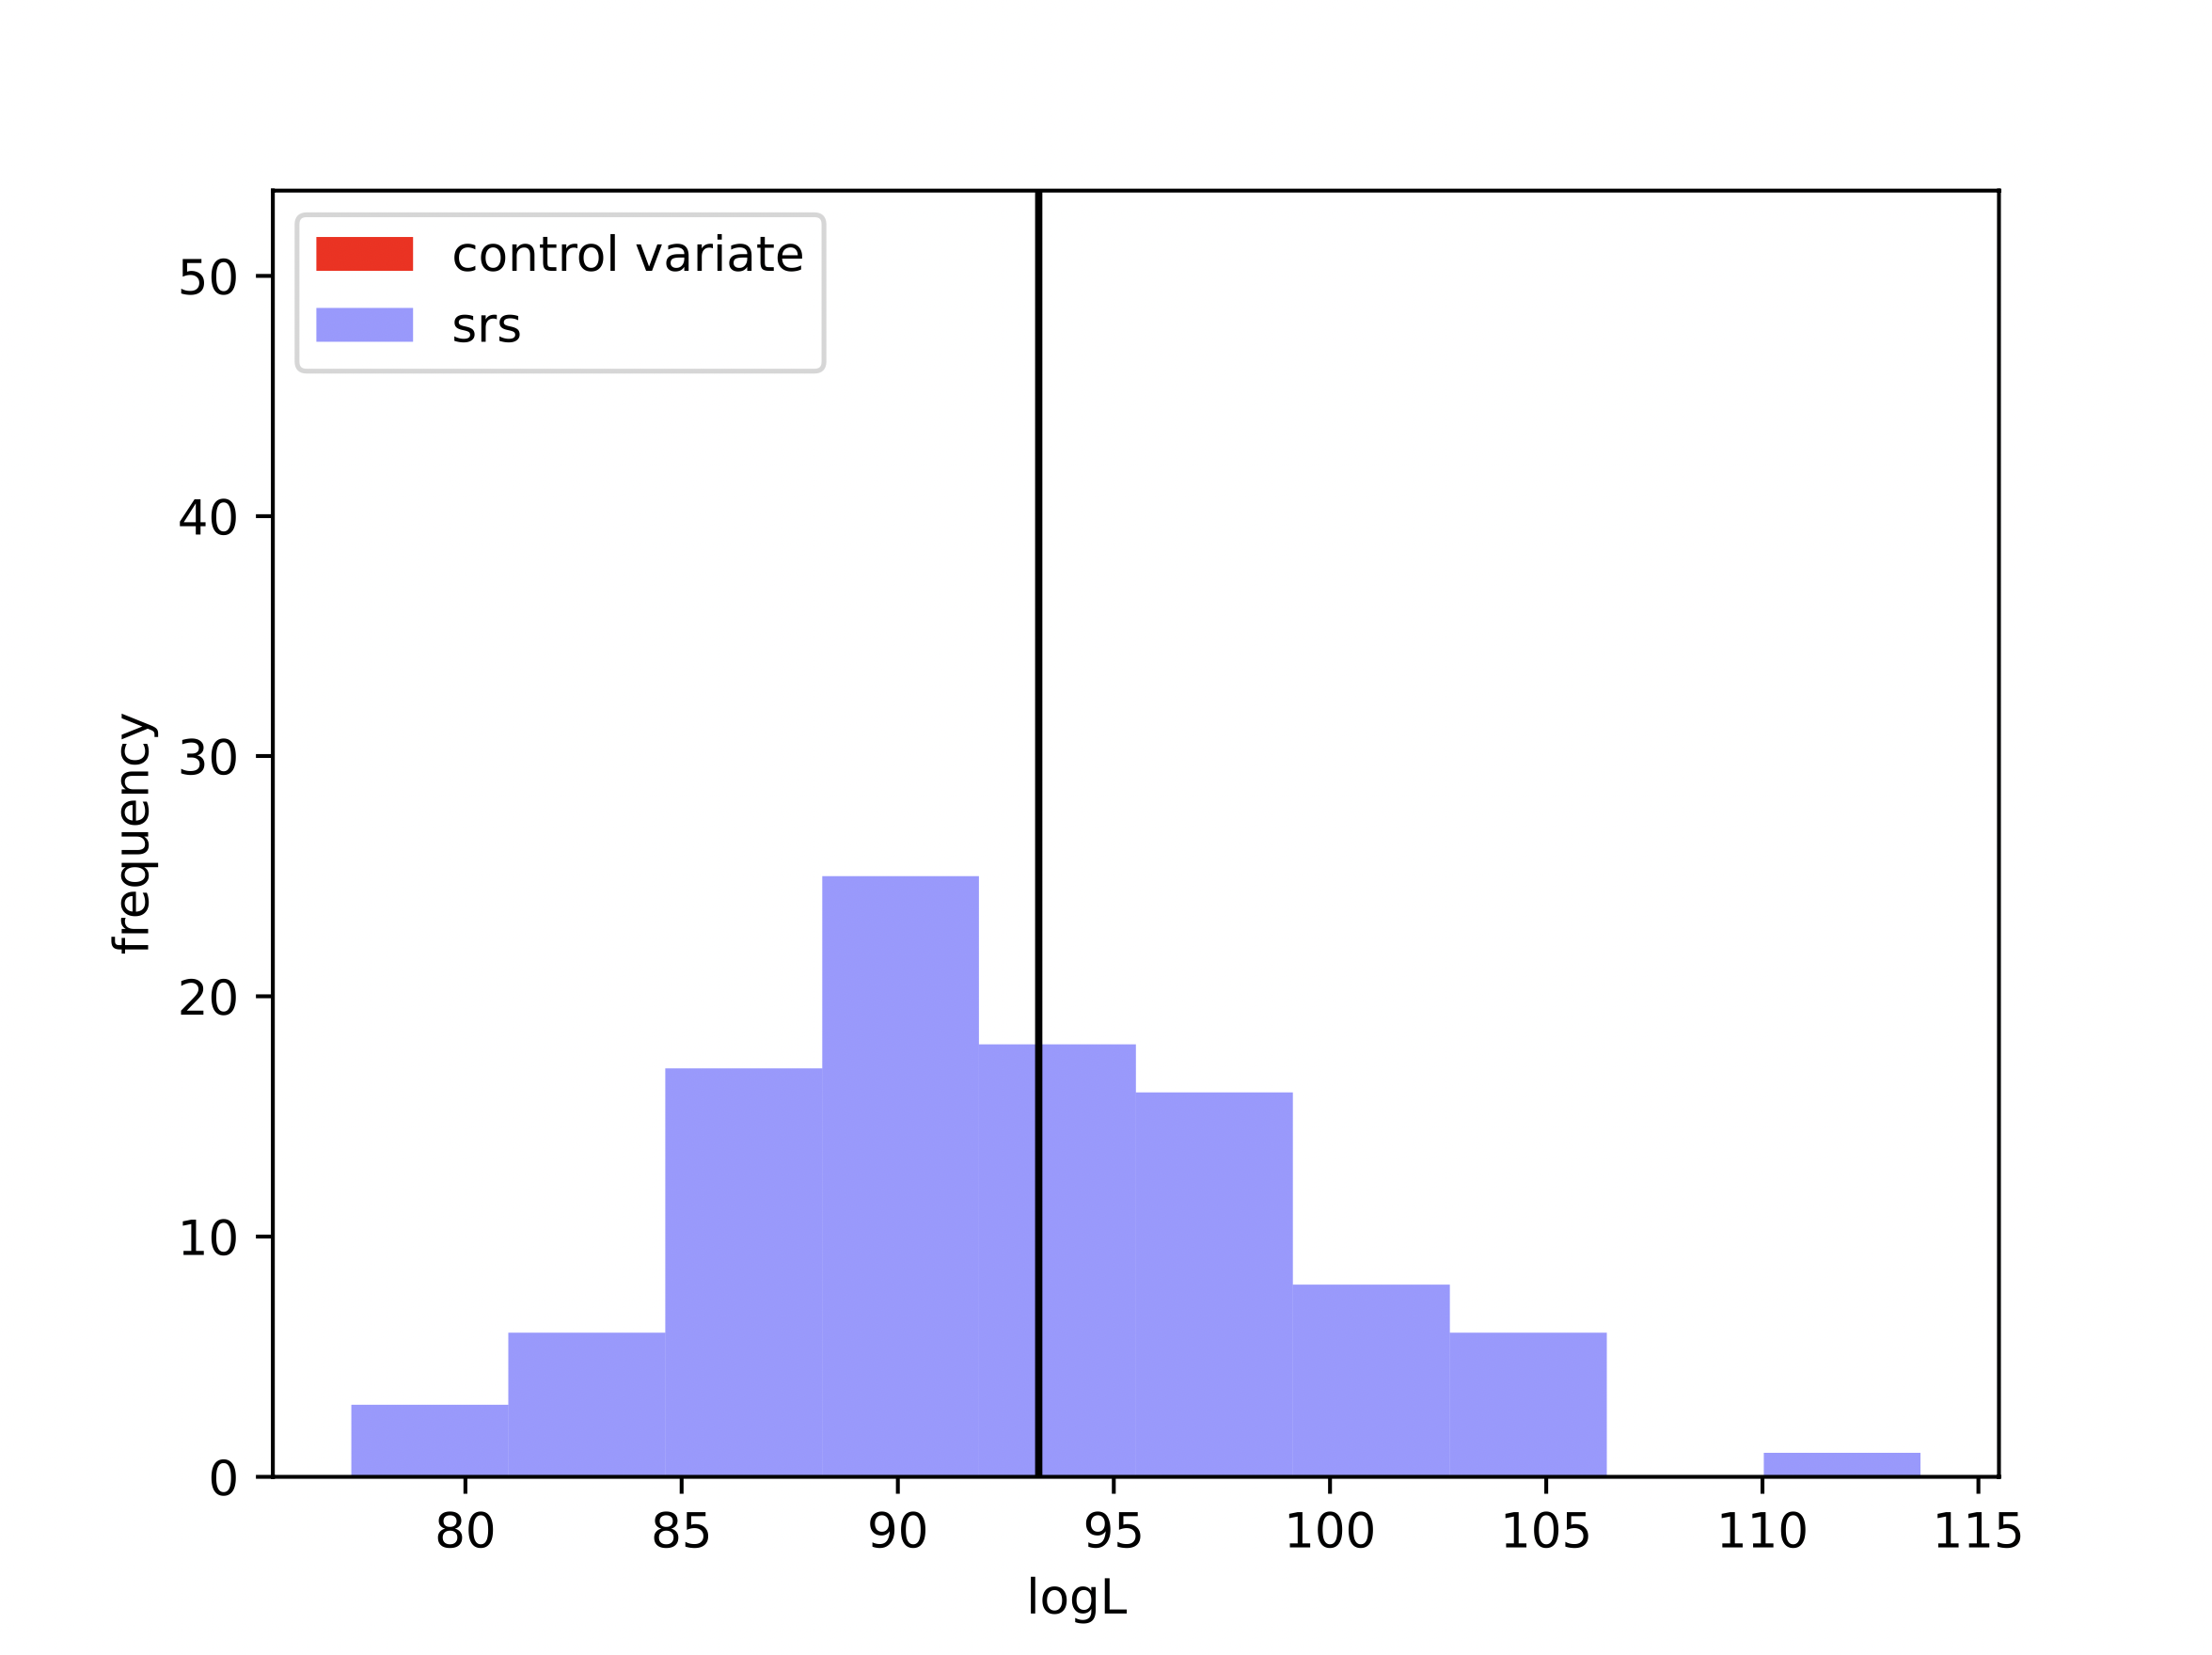
\includegraphics[width=1.0\textwidth]{Chapter3/Figs/regen3_28.png}
\caption{ The plotted histograms represent the total log-likelihood values for the linear $f(x,\theta)$ mentioned above in \cref{eq:strt}. There are 100 $\log L(\theta)$ samples plotted for both histogram plots. The $\theta$ chosen for these subsamples of $\log L(\theta)$ are the true values of the parameters of our model. These are namely $b=2$ and $c=1$, referring to \cref{eq:strt}. The black vertical line represents the true value of the total log-likelihood. The blue histogram represent the values estimated by the SRS method (without control variates). The values estimated by control variate subsampling are also plotted on the figure as red histograms but, as expected, they cannot be seen at the scale of this graph. This is because, beyond machine precision, there is no noise in the control variate subsampling log-likelihood values as the underlying function is linear. This is analogous to the mean and standard deviation being sufficient statistics to reconstruct a dataset.}
\label{fig:two}
\end{figure}

Having built an intuition regarding the meaning of the `hyperparameters'--$K$, $m$, and $n$--and their relation to the `model' and data, we move towards analysing the results produced by control variate subsampling as applied to this concrete example case of a Gaussian likelihood with a linear function as the `model'. Consider that we approximate the total log-likelihood with SRS, as in \cref{eq:fgf}. We set the number of subsampled points, $m$, to 55 and repeat this log-likelihood approximation $100$ times--each time choosing a different randomly selected subsample of 55 points from the $n=100$ total. Consider, that we also try to approximate the total log-likelihood with control variate subsampling, as in \cref{cvv}. We repeat this process 100 times as well. To maintain a like-for-like comparison, we try to keep the computational cost constant for both control variate subsampling and SRS. We can do this by choosing the following hyperparameters for the control variate subsampling case: number of clusters, $K=5$, and the number of subsamples, $m=20$. We go into further detail regarding the computational costs and how we arrive at these numbers in the \cref{sec:computational_costs} `Computational Costs'. The reader should keep in mind that this is the trivial case due to it being a linear function and the Taylor expansions in the control variates being second order. Thus the control variates subsampling ends up being analytically equal to the full raw dataset likelihood sample. We plot all these results as histograms in the \cref{fig:two}.


We now move onto a non-trivial case in order to show the effect of subsampling where
%
\begin{equation}
    f(x_i,\theta) = bx_i^3+ c.
\label{eq:tertiary poly}
\end{equation}
%
As emphasised before, there are several different moving parts to the control variate method, so we shall again try to build further intuition. We plot the function from \cref{eq:tertiary poly} in data-space in \cref{fig:three}, along with all the other `hyperparameters' of the method itself--$K$, $n$ and $m$. Such that everything is visualised . Note that for the purpose of the figure we give the following numerical values to the hyperparameters for less visual clutter: $K=5$, $n=100$, and $m=20$.
%
\begin{figure} 
\centering    
\includegraphics[width=1.0\textwidth]{Chapter3/Figs/Raster/fig3_30.pdf}
\caption{ This graph illustrates the control variate subsampling method described by \cref{cvv}--it aids the reader to better understand what the `hyperparameters', $K$, $m$, and $n$, mean. Our randomly uniformly generated data points $\textbf{z}_i= \{x_i,y_i \}$, plotted with the axes representing the $x$ and $y$ coordinates. The 5 red squares represent the cluster centres, according to which each point is classified and then colour coded appropriately. The blue line through the centre of the points is the function $f(x,\theta)= bx^3+c$. We have $100$ data points plotted in total. The $m$ referred to in \cref{cvv} would be some randomly chosen subsample. These are unrelated to the $K$-clusters. These $m$ points are visualised by the points, among the $100$ data points, that are marked by the black crosses on top of them.}
\label{fig:three}
\end{figure}
%
It is also insightful to compare the gradients and Jacobians corresponding to the linear and third degree polynomial functions that go into evaluating the control variates. For the linear case:
%
\begin{align}
   \nabla_z l(\bar{\textbf{z}}_{k_{i}},\theta) &= \frac{1}{\sigma_{k_{i}}^2} \begin{pmatrix}(y_{k_{i}}-bx_{k_{i}}-c)b\\-(y_{k_{i}}-bx_{k_{i}}-c)\end{pmatrix},\\
   \nabla_z \nabla_z l(\bar{\textbf{z}}_{k_{i}},\theta) &=  \frac{1}{\sigma_{k_{i}}^2} \begin{bmatrix}
-b^2 & b \\
b & -1 \\
\end{bmatrix}
\end{align}
%
Correspondingly for the third degree polynomial function:
%
\begin{align}
   \nabla_z l(\bar{\textbf{z}}_{k_{i}},\theta) &= \frac{1}{\sigma_{k_{i}}^2} \begin{pmatrix}(y_{k_{i}}-bx_{k_{i}}^3-c)(3bx_{k_{i}}^2)\\-(y_{k_{i}}-bx_{k_{i}}^3-c)\end{pmatrix},\\
   \nabla_z \nabla_z l(\bar{\textbf{z}}_{k_{i}},\theta) &=  \frac{1}{\sigma_{k_{i}}^2} \begin{bmatrix}
9b^2x_{k_{i}}^4+(y_{k_{i}}-bx_{k_{i}}^3-c)(6bx_{k_{i}}^2) & 3bx_{k_{i}}^2 \\
3bx_{k_{i}}^2  & -1 \\
\end{bmatrix}
\end{align}
%
As we plot the results for the third degree polynomial case in \Cref{fig:gggh}, we select $n=10,000$. We select $m=300$ for the SRS case. For the control variate method we select $K=20$, and $m=160$--again keeping the computational costs equivalent for both. This time, however, instead of $100$ different calculations of the total log-likelihood estimation, we gave each method $1000$ runs so that there is more certainty on the variance values we extract.



\Cref{fig:gggh} shows that the control variate method significantly improves upon simple random sampling. Further, it becomes increasingly favourable over SRS as we increase $n$ and decrease $m$. This is fortunate since the larger the dataset the more likely we are to need to resort to subsampling. The smaller our capability of subsampling then the more favourable this method becomes. In other words, the fewer resources one has in comparison with the magnitude of the computational costs, the better the method becomes in comparison with simple random sampling. We found that for SRS to compete with control variate subsampling it needed on the order of five times as much computational cost to produce equivalent precision. 





\begin{figure} 
\centering    
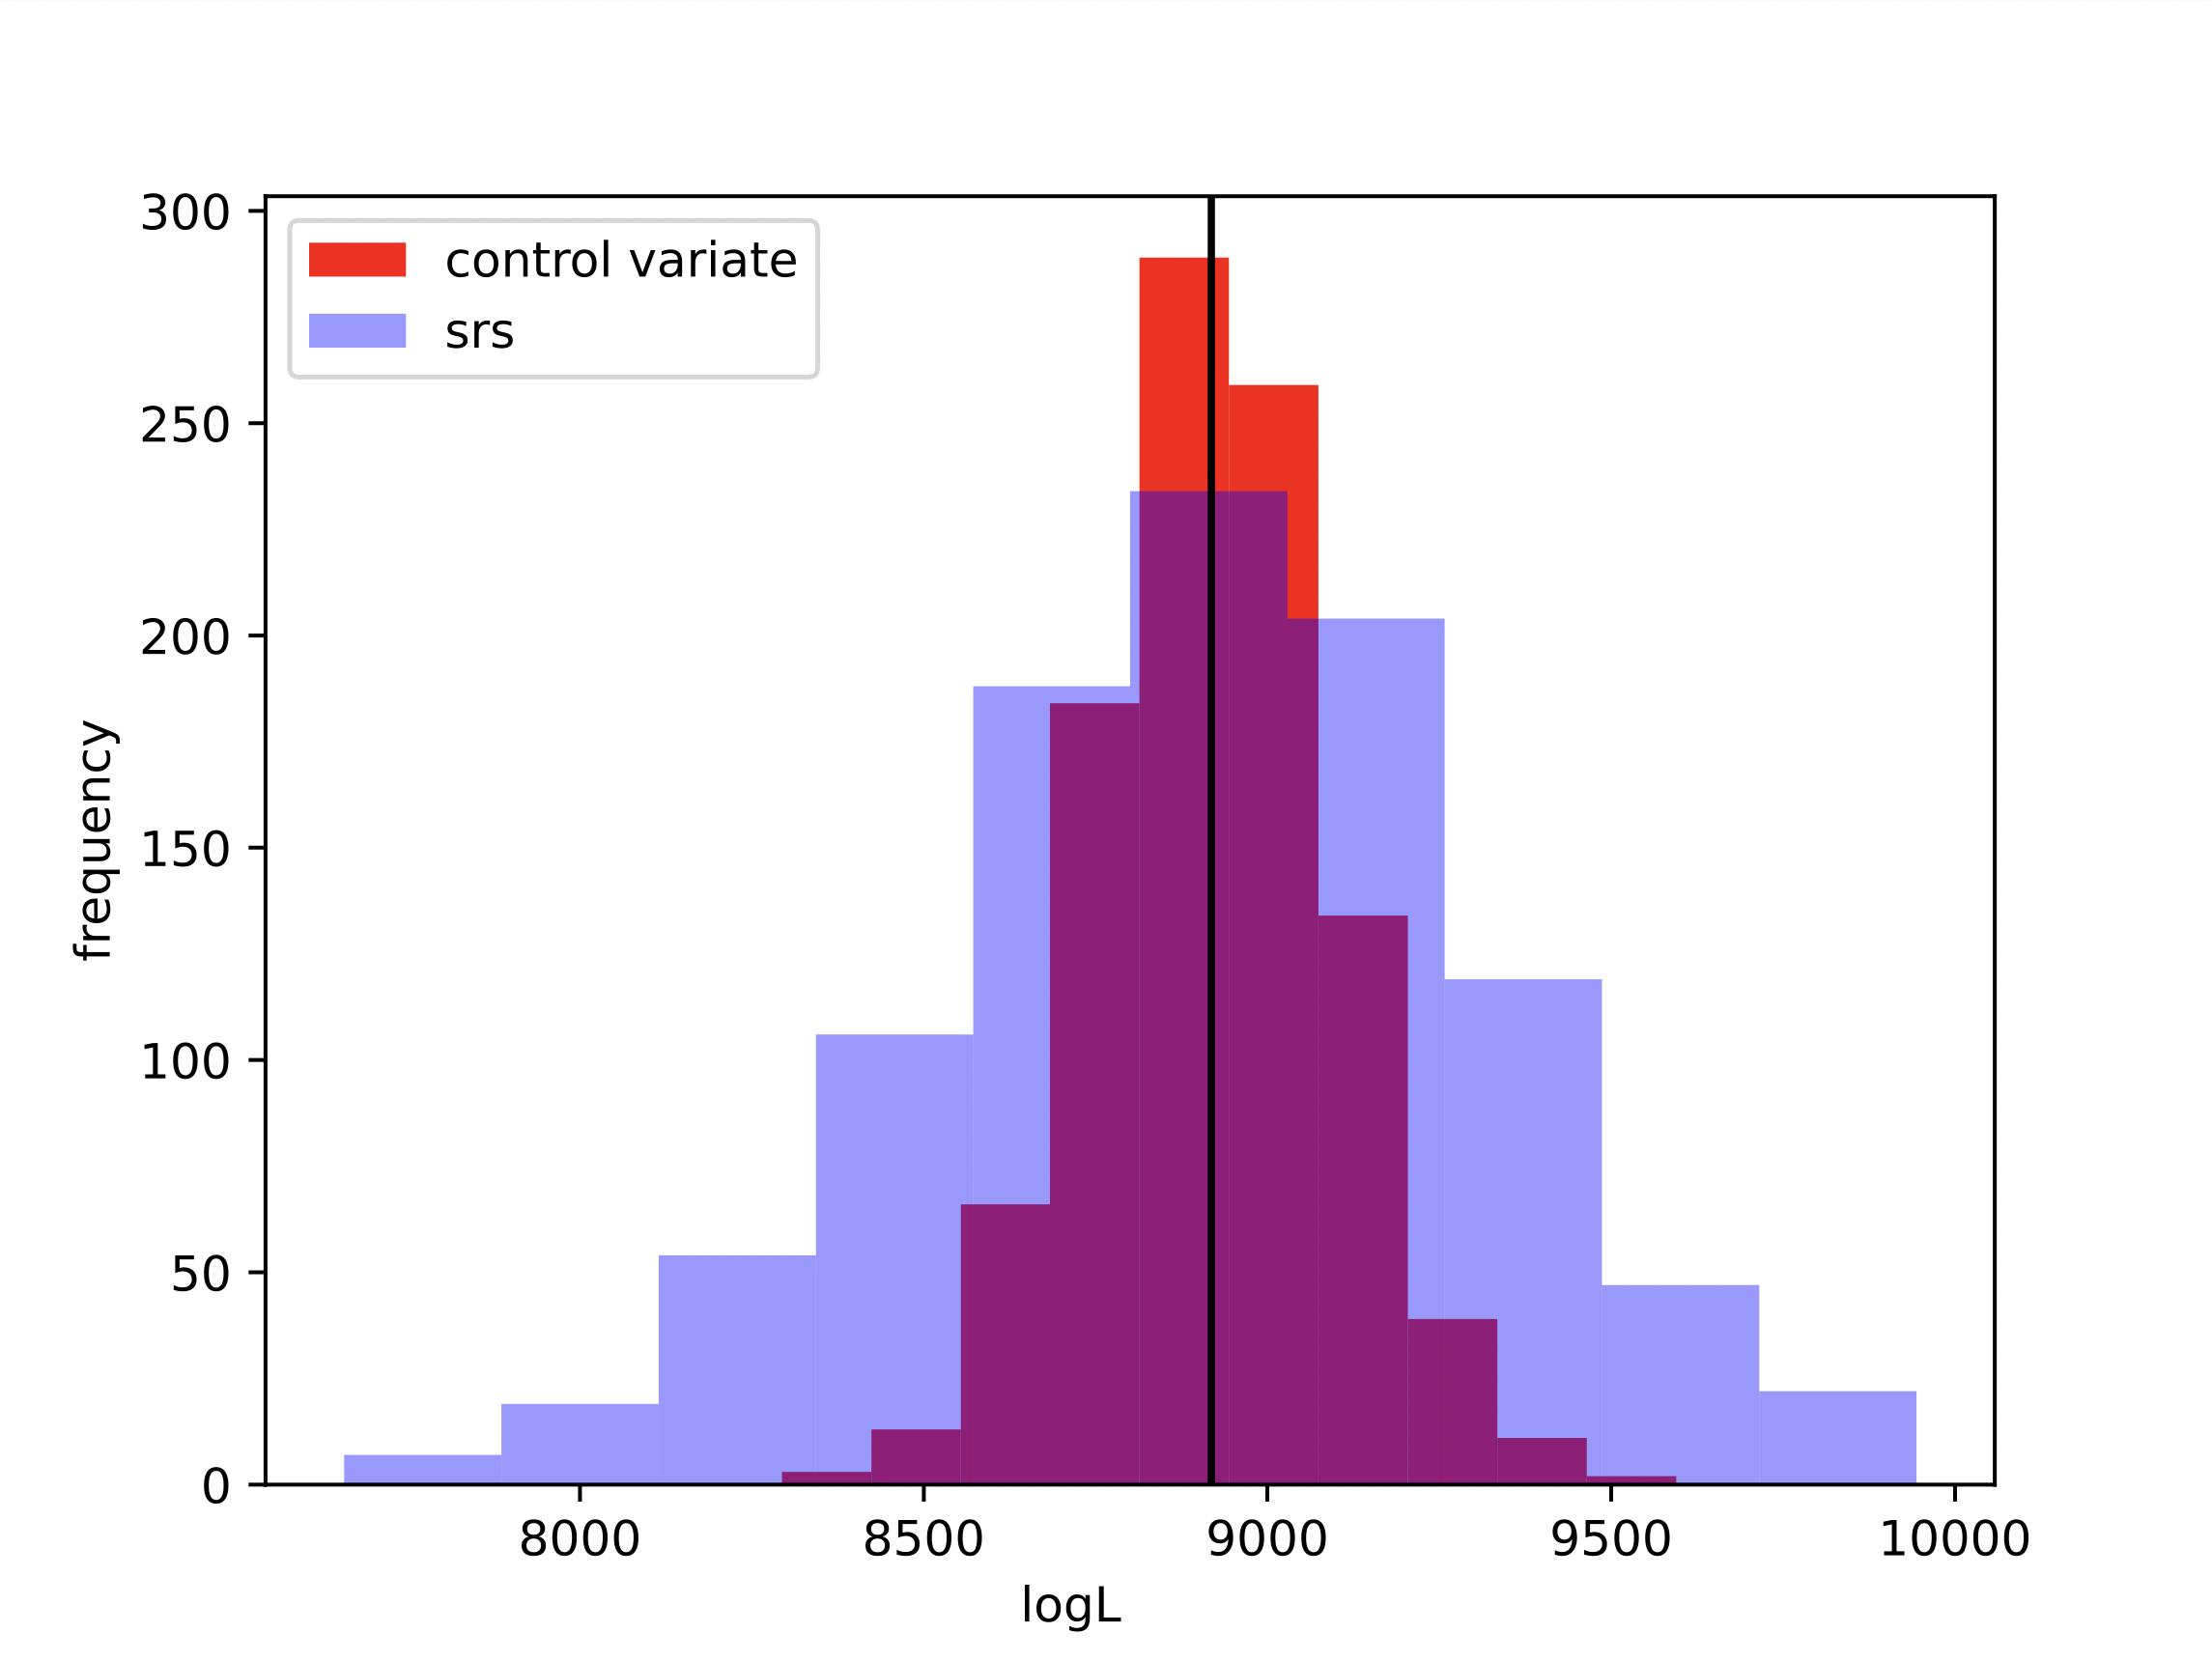
\includegraphics[width=1.0\textwidth]{Chapter3/Figs/regen3_29.png}
\caption{ The plotted histograms represent the total log-likelihood values for the third degree polynomial $f(x,\theta)$ mentioned above in \cref{eq:tertiary poly}. There are $100$ $\log L(\theta)$ samples plotted for both histogram plots. The $\theta$ chosen are the true values of the parameters of our model, namely $b=2$ and $c=1$, referring to \cref{eq:tertiary poly}. The black vertical line represents the true value of the total log-likelihood. The blue histogram represents the values estimated by the SRS method without control variates. The control variate subsampling method produces the red histogram. The control variate method is significantly superior to simple random sampling in these results. The standard deviation of the results given by the control variate method is $2.5$ times less than the simple random sampling.}
\label{fig:gggh}
\end{figure}

In this section the control variate subsampling method has been applied to a toy function, $f$. Now let us look into further detail regarding the computational costs of this method.


\subsection{Computational Costs}\label{sec:computational_costs}
In the Quiroz et al. paper~\cite{Quiroz_2018}, the computation costs of evaluating \cref{cvv} were quoted as
%
\begin{equation}
\mathrm{cost} = K \cdot c_{\bar{l}} + m \cdot c_{l}.
\end{equation}
Here  $c_{\bar{l}}$ is the computational cost of evaluating a control variate, $c_{l}$ is the cost of evaluating a single log-likelihood contribution, $m$ is the number of subsamples and $K$ is the number of cluster centres. Note, we only need to allocate the points to their respective clusters once, and evaluate the $(z_i-\bar{z_{k_i}})$ terms in \cref{cvv} once. We only need to do these once because this is at the data level, which is fixed--rather than the parameter level, which vary throughout the fit. This effectively renders only $K$ unique $\bar{l}$ terms to be evaluated for the whole dataset at each MCMC or nested sampling iteration.

Since $K \ll m,n$, this shows that the computational costs are roughly equivalent to SRS with a similar $m$--all while producing much more accurate results (Assuming $c_{\bar{l}} \approx c_{l}$ which is not unreasonable). In the common case of a Gaussian-distributed error on the response variable, the computational cost relationship is 
%
\begin{equation}
    c_{\bar{l}} \approx 7*c_{l}.
\end{equation}
%
This is since that $l(\bar{\textbf{z}}_{k_{i}},\theta)$ in \cref{eq:taylor} has $1$ independent sum; $\nabla_z l(\bar{\textbf{z}}_{k_{i}},\theta) \cdot (\textbf{z}_i-\bar{\textbf{z}}_{k_{i}})$ has $2$ sums since it is a vector dot product; and, finally, $\frac{1}{2}(\textbf{z}_i-\bar{\textbf{z}}_{k_{i}})^\intercal  \nabla_z \nabla_z l(\bar{\textbf{z}}_{k_{i}},\theta)(\textbf{z}_i-\bar{\textbf{z}}_{k_{i}})$ has $4$ independent sums, since it goes from a matrix to a scalar. For concreteness we shall be more explicit in what we mean by independent sums. When we say 4 separate sums for $\frac{1}{2}(\textbf{z}_i-\bar{\textbf{z}}_{k_{i}})^\intercal  \nabla_z \nabla_z l(\bar{\textbf{z}}_{k_{i}},\theta)(\textbf{z}_i-\bar{\textbf{z}}_{k_{i}})$ we mean that once we carry out this matrix multiplication there are 4 independent `numbers' that we have to sum up to get the value. These all add up to $7$ separate terms. This is in comparison with each log-likelihood only having $1$ separate term. Thus for the computational costs to align we had the constraint,
%
\begin{equation}
    K \cdot 7 + m_{\textrm{Control Variate}}= m_{\textrm{SRS}}.
\end{equation}
%
Here $m_{\textrm{Control Variate}}$ and $m_{\textrm{SRS}}$ are the $m$s used in the control variate and SRS methods respectively (refer to what we label $m$ in \cref{eq:fgf} and \cref{cvv} respectively). 



\subsection{Voronoi Cell Averaged Subsampling Comparison with Control Variate Subsampling}\label{sec:voronoi}


We have shown promising results suggesting that control variate subsampling may be better than SRS in some cases. However, for the purpose of this thesis we must also compare with results the Voronoi cell averaged subsampling technique used in \cite{Mihaylov_2020}. Doing so will support our main assertion in \Cref{ch:chapter4}: that our newly proposed control variate subsampling method will ideally improve the accuracy of the Bayesian analysis performed in the gravitational wave detection technique in the original paper \cite{Mihaylov_2020}. This paper uses the aforementioned Voronoi subsampling method for sampling likelihoods. Briefly, Voronoi cell averaged subsampling consists of clustering all the data points by the Voronoi cells--i.e.\ labelling them to the Voronoi cell that they are closest to in data-space--then, averaging over all the points in a Voronoi cell to get a Voronoi cell average. After this is performed, for every subsequent sample of the likelihood function, this average value average value of the data of a particular Voronoi cell is then used in place of every point that exists within the Voronoi cell. This evidently results in a deterministic likelihood. For further detail refer to \cite{Mihaylov_2020}.


Since Voronoi cell averaged subsampling is completely deterministic we cannot repeat the comparisons performed in \cref{fig:gggh} again to analyse its utility. It would not produce a histogram with a spread as seen in \cref{fig:gggh}, but rather a simple vertical line due to its deterministic nature. A better comparison would be of the accuracy of the resulting $\log Z$ values produced by each sampling method for the Bayesian analysis performed on the third degree polynomial `model' from \cref{eq:tertiary poly}. The evidence values were calculated by carrying out orthodox nested sampling--but in place of the usual likelihood we plugged a non-deterministic likelihood generated by one of the subsampling methods. For all three subsampling methods, SRS, Voronoi cell average subsampling, and control variate subsampling, we shall use `hyperparameters'--$n$, $m$ and/or $K$--which result in equivalent computational cost for all 3 sampling method runs, to produce a like-for-like comparison. The total number of data points used were $n=10,000$. The number of Voronoi cells was $300$ and similarly the subsample size $m$ for SRS was $300$ at each subsample. To get the equivalent computational cost for a control variate subsample we must set $k=22$ and $m=146$; where we used the computational cost calculations from the previous section.



\begin{table}[h!]
\begin{center}
\begin{tabular}{c|c}
Method                              & $\log Z \pm \sigma$ \\
\hline
Voronoi cell average subsampling    & $13,597 \pm 0.4$    \\
SRS                                 & $9,105 \pm 0.7$     \\
control variate subsampling         & $8,920 \pm 0.8$     \\
deterministic full dataset sampling & $8,850 \pm 0.4$    
\end{tabular}
\end{center}
\caption{Log-evidence values produced by the different subsampling methods\label{tab:subsampling}}
\end{table}

We can see that not only did control variate subsampling outperform the Voronoi subsampling method used in \cite{Mihaylov_2020}, but so did simple random subsampling. Control variate subsampling was by far the closest in producing the correct $\log Z$ value--which is labelled by ``deterministic full dataset sampling'' in \cref{tab:subsampling}. This yet again shows that, if we can get past the turmoil related to the unsuitability with non-determinism of the current nested sampling packages, we are far better off dealing in non-deterministic subsampling rather than deterministic. The reason papers in the literature, such as Ref \cite{Mihaylov_2020}, widely avoided non-determinism was not because it is less accurate. Rather they avoided it because none of the widely used nested sampling packages could cope with non-determinism. Thus, in the next section we show how to implement non-deterministic log-likelihoods into nested sampling in the following section.

Note that the \cref{tab:subsampling} shows favourable results for control variate subsampling over the Voronoi averaging method. This is true even though the particular model and data we were dealing with, were as favourable as it gets for Voronoi averaged subsampling. Even with all the advantages of a suitable problem, Voronoi subsampling still significantly underperformed control variate subsampling. The reason for this being an advantageous problem for Voronoi subsampling is that the variation of the data spanned within a particular Voronoi cell is minute. The range spanned by our data is $x=[-1,1]$, and within this small region are packed $300$ Voronoi cells. Another requirement given in \cite{Mihaylov_2020} for the Voronoi subsampling method to be maximally accurate is that the error associated with each data point has to be independent from the others. This requirement is built into our toy model. Yet, the control variate subsampling still produced more favourable results. Note, as well, that our subsamples $m$ were only on a scale of roughly $30 \times$ smaller than the total dataset $n$. 





\section{Which Nested Sampling Algorithm is Best Suited to Tackle Non-Determinism?}\label{sec:nondet}

In exploring how to accurately implement nested sampling on non-deterministic likelihoods we tried the implementation of multiple versions of nested sampling algorithms. It is not clear to what extent the nested sampling meta-algorithm is valid for non-deterministic likelihoods. However, we made some preliminary investigations that are the subject of ongoing research.


\subsection{How We Simulated Non-Determinism}
The way we generated ``non-deterministic'' likelihoods was by first generating the dataset of $\{x_i,y_i\}$. The model for $y$ that we are trying to test our model that was
\begin{equation}
F(x)= bx+c.
\end{equation}
This function acts as our ``theory model''--analogous to an equation of a physical theory we may be testing against data. It has two parameters that we seek to find out the true value of--$\theta = [b,c]$. $\{x_i\}$, was generated by drawing them uniformly between $-1$ and $1$. Then by taking a randomly selected subset of this dataset $\{x_i\}$ and feeding it again into the function above, $F(x_i)$, we generated the subsample that generates a non-deterministic log-likelihood:
%
\begin{equation}
    \log L = \frac{n}{m}\sum_j^m -\frac{\log (2\pi\sigma^2)}{2} - \frac{ (y_j - F(x_j)^2}{2\sigma^2}.
\end{equation}
%
Here, $n$ is the size of the full raw dataset, $m$ is the size of the selected subsample of the dataset, $j$ is the dummy variable we sum over. For the non-deterministic runs of nested sampling, whenever we sample the log-likelihood we have a newly randomly selected subset $x = \{ x_{k_0}, x_{k_1},...,x_{k_m}\}$ of the full dataset $x= \{ x_0,x_1,...,x_n \}$ to get a dataset of $F(x_i)$. At each call of the log-likelihood function in the code by nested sampling, such a new sub-dataset is used to generate the non-deterministic log-likelihood. Depending on which random subset is sampled from the full raw dataset, the same parameters choice, $\theta$, may yield different log-likelihood values.



\subsection{Bayesian Evidence of Non-deterministic Likelihood}


\begin{figure} 
\centering    
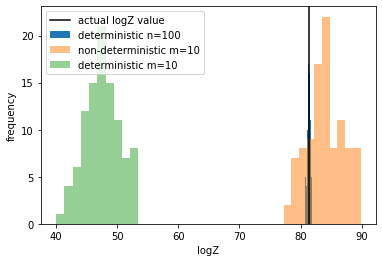
\includegraphics[width=1.0\textwidth]{Figure 2022-09-02 221530}
\caption[Orthodox]{Histograms of log Z values from Metropolis Hastings nested sampling. The deterministic likelihood using the full dataset produced the most ideal results. The non-deterministic likelihood produced evidence values that were less accurate but contained the true value within their error margin. However, the deterministic likelihood that did not use the full dataset, represented by the green histogram, did not even contain the correct values within the distribution. There are 100 $\log Z$ values plotted in each histogram.}
\label{fig:logZ2}
\end{figure}

\begin{figure} 
\centering    
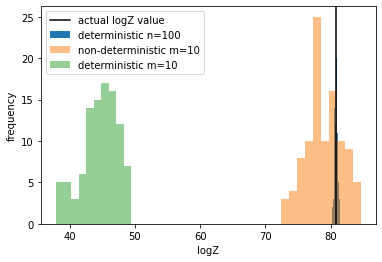
\includegraphics[width=1.0\textwidth]{logz_hist_orthodox1}
\caption{Histograms of $\log Z$ values from orthodox nested sampling. Again, the deterministic likelihood using the full dataset produced the most ideal results. The non-deterministic likelihood produced evidence values that were less accurate but contained the true value within their error margin. However, the deterministic likelihood that did not use the full dataset, represented by the green histogram, did not even contain the correct values within the distribution. The exact true value of $\log Z$ is plotted for reference as well as the black vertical line. There are 100 $\log Z$ values plotted in each histogram. }
\label{fig:logZ11}
\end{figure}


All 100 of the $\log Z$ values in \cref{fig:logZ11} are derived from a single set of $\log L$ values. This is to be as true to the circumstances we would find in the real world where the computationally limiting factor is sampling the $\log L$ values. Simulating the corresponding sets of $\log X$ values to go along with this one set of $\log L$ values is computationally trivial in comparison, thus these 100 $\log Z$ values come from one set of $\log L$ values paired with 100 sets of simulated $\log X$ values. We can see that the deterministic subsample is far off mark, as expected. The non-deterministic subsample run fares much better. As expected the variance of the log-evidence values from the full dataset is far smaller than the from the subsamples.


The Metropolis Hastings nested sampling works nearly the same as orthodox nested sampling except with an altered mechanism of suggesting a new live point at each iteration. Instead of completely randomly selecting new points from the same domain until one satisfies acceptance criteria, we start with an already acceptable live point and take a `random walk' starting from there. In our version of Metropolis Hastings nested sampling, we propose a new point by: identifying the live point corresponding to the lowest likelihood, taking a number of steps as increments in the parameter space, and only accepting a proposed step if it has gone in a direction of increasing log-likelihood in parameter space. The step looks like this:
%
\begin{equation}
\theta_\mathrm{old}=\theta_{\mathrm{new}}+\epsilon.    
\end{equation}
%
Here, $\epsilon$ is selected as a random variable vector distributed as a normal distribution with mean zero and covariance equal to the covariance of the parameter space dataset of current live points.

We believe that Metropolis Hastings is inherently better suited to deal with non-determinism due to its step by step walk which allows it to stay within the allowed iso-likelihood contours even in the midst of large log-likelihood function uncertainty. This is supported by our preliminary testing, in which we found Metropolis Hastings nested sampling to converge quicker than orthodox nested sampling while achieving a similar level of accuracy.



\subsection{Stopping Criteria}
Non-deterministic likelihoods require significant care into the choice of a stopping criteriion. The stopping criterion that we implemented was that if the mass contributions, $ Z_n = L_nw_n$, to of the cumulative evidence up until the latest iteration, $ Z = \sum_i^n L_iw_i$, was smaller than some given tolerance,
\begin{equation}
\frac{ Z_{n}}{ Z}< \epsilon_{\mathrm{tol}}
\end{equation}
 for five consecutive nested sampling steps, then the algorithm would terminate. The idea behind this is that continuing the algorithm will experience diminishing returns after some point such that the contributions to the evidence are consistently below some threshold that we deem appropriate. The reason we require that this happens 5 times consecutively is that due to the probabilistic nature of nested sampling, we may erroneously encounter a small increment in evidence mass. This doesn't necessarily mean that the actual posterior mass increments are going to be small then-on, but if it happens 5 times in a row then it likely was not due to a chance event.

 Our stopping criterion is somewhat of a proxy for that which is generally used in the nested sampling literature, the approximate remaining evidence by total accrued evidence. \texttt{MultiNest} and \texttt{PolyChord} both use estimators of this and set a tolerance for the fraction of estimated remaining posterior mass. \texttt{PolyChord} has the break condition:
%
 \begin{equation}
\bar{L}(1-X_i)/Z=\Delta Z/Z<\mathrm{tol},
 \end{equation}
%
 where $\bar{L}$ is the average likelihood taken from all the samples. We found this breaking criterion to be perhaps too stringent in the case of non-deterministic likelihoods. We find that significant noisiness in the likelihood may cause uncharacteristic oscillations in the accumulated evidence at each iteration which would prevent termination of nested sampling indefinitely. Perhaps this is among the reasons \texttt{MultiNest} and \texttt{PolyChord} struggle. However this is not a conclusive remark and more work needs to be done on this. Trying to counter this one may reduce the tolerance to a significant degree. However, when the magnitude of non-determinism becomes too large we may also find that we may make increments in the evidence that are uncharacteristically low, causing premature termination of the algorithm. In such circumstances we chose to put a hard constraint of total number of nested sampling algorithm iterations before algorithm termination. Trial and error may be used to determine an appropriate value for the number of iterations before termination.

 \subsection{Summary of Compatibility of Various Nested Sampling Algorithms with Non-deterministic Likelihoods}

 A summary of our preliminary explorations:



\begin{enumerate}
    \item \texttt{PolyChord} is a nested sampling algorithm that uses slice sampling. Slice sampling consists of sampling within a likelihood bound using an already existing live point and a guess of the bound size. This sampling method completely failed to converge. \cite{Handley_2015} This is because slice sampling assumes a deterministic likelihood, and therefore would never work. Slices regularly fail to to terminate under a likelihood that fluctuates and changes the bounds of a slice.

     \item Our own orthodox nested sampling that we coded from scratch converged, as can be seen in \cref{fig:logZ11}. Orthodox nested sampling uses `brute force' rejection sampling from the unit hypercube until a point is found within it. This is therefore not generally scalable but for the small problems we consider here acts as a good point of reference. 
    \item \texttt{MultiNest} uses rejection sampling from the unit hypercube as well. Its rejection sampling quickly breaks down as soon as the non-determinism becomes significant and, thus, fails to converge~\cite{Feroz_2009}. As alluded in the section above, we believe that this may be due to their choice of stopping criterion.
   
    \item Our own Metropolis Hastings nested sampling coded from scratch, which used a random walk from an already existing live point to sample new points. Our algorithm consistently converged. This is shown in \cref{fig:logZ2}. \cite{doi:10.1080/00031305.1995.10476177}
\end{enumerate}

\section{Conclusions}


Our main conclusion is that all of our results show non-deterministic subsampling performs favourably over deterministic subsampling. Theoretically this should be true given that the number of times the subsamples are drawn is sufficient, which we believe is often the case for MCMC and nested sampling. Several results across this chapter suggest this. Our major contribution is not only in introducing to the astronomy scientific community an improvement to SRS, in efficient subsampling through control variates, but also in showing how simple non-deterministic likelihoods can actually be made viable for nested sampling. To the best of our knowledge, this incorporation of non-deterministic likelihoods in nested sampling has not been examined in the astrostatistics literature before this thesis. Regarding control variate subsampling, the control variates, from \cref{eq:taylor}, encompass the information encoded in the global landscape of the log-likelihood over all of data-space. The control variate subsampling scheme also accounts for local effects and thus has the same local precision benefits as SRS, since it not only has a Taylor series spanning the whole data space, but also local subsamples as in SRS. This contributes towards making control variate subsampling a robust method. The Taylor expansion terms--first sum in \cref{cvv}--give a picture of the general macro-structure and information encoded within the log-likelihood manifold over the whole of the data space. On top of this, the subsampling terms--the second sum in \cref{cvv}--give a localised view of the smaller scale structures. The accuracy and precision of control variate subsampling as compared to SRS grows as the ratio $n/m$ grows. So, for big data, such as cosmological datasets, stock market data, large language model training datasets etc., control variate subsampling becomes increasingly favourable as the task becomes more data-intensive.


%!TEX root = ../thesis.tex
%*******************************************************************************
%****************************** Third Chapter **********************************
%*******************************************************************************
\chapter{Control variates, Gaia downsampling and gravitational waves}\label{ch:chapter4}

% **************************** Define Graphics Path **************************
\ifpdf
    \graphicspath{{Chapter4/Figs/Raster/}{Chapter4/Figs/PDF/}{Chapter4/Figs/}}
\else
    \graphicspath{{Chapter4/Figs/Vector/}{Chapter4/Figs/}}
\fi

\section{Gravitational waves}
Cosmological datasets are among the most data-intensive in the realms of numerical science. Thus they are a prime example of the utility of the control variate subsampling method. The particular example we shall look at to demonstrate this is an astrometric search method for individually resolvable gravitational wave sources with Gaia~\cite{Mihaylov_2020}. To introduce this, we must describe the astrometric response of stars to gravitational waves. Essentially, we can detect gravitational waves by measuring deflections of apparent star positions in the sky which correspond to gravitational waves deflecting the photons when they are emitted by the star and when they are measured at Earth. We shall examine both circumstances where the star term is included and where we can use a far-field limit that ignores the star term.

This astrometric search method was first suggested by \cite{VB}, and first derived by \cite{1996ApJ...465..566P}. Consider a metric perturbation, $h_{\mu \nu}$, due to monochromatic gravitational wave that can be written out as
%
\begin{equation}
h_{\mu \nu}(t,\textbf{x})= H_{\mu \nu} \exp( ik_{\rho}x^{\rho } )
\end{equation}
%
where $H_{\mu \nu}$ are the small complex constants satisfying transverse-traceless gauge conditions, the wavevector $k^{\mu} = (\omega, -\omega \textbf{q})$ is null, and $\textbf{q}$ is the direction unit vector of the monochromatic plane-fronted gravitational wave. Using this metric tensor one can derive the following expression for the astrometric deflection of a star as measured at Earth~\cite{Mihaylov_2020,1996ApJ...465..566P}:
%
\begin{equation}
\delta n_i = \frac{(n_i - q_i) h_{jk}(E)n^j n^k}{2(1-\textbf{q} \cdot \textbf{n})}-\frac{h_{ij}(E) n^j}{2},
\label{eq:earthterm}
\end{equation}
%
where the $n_i$ terms refer to star coordinates, and $h_{ij}(E)$ are the metric perturbations at the Earth--referred to as the ``Earth term". This expression is true at the far-field limit. Now consider a star with coordinates $(x,y,z)$, where the Earth is at the origin of this coordinate system. We label a photon emitted from this star as having spatial direction $\propto (p^x,p^y,p^z)$. Consider also a $+$ polarisation gravitational wave travelling down the $z$-axis with $A$ amplitude and $\omega$ frequency. This is without loss of generality as a simple coordinate transform could always align the $z$-axis with the gravitational wave, and the $(x,y)$ axis with the $+$ polarisation. Using \cref{eq:earthterm} this essentially translates to the apparent star positions, as observed from the Earth, being~\cite{Lasenby_2019}:
\begin{align}
    \frac{p^x}{p^z} &= \frac{x}{z}-\frac{A x \left(r z +x^2-y^2+z^2\right)\cos \left(\left(r + t \right) \omega \right) }{\omega^2 \left(r +z \right) z^2} \label{eq:px}\\
    \frac{p^y}{p^z} &= \frac{y}{z}+\frac{A y \left(r z -x^2+y^2+z^2\right)\cos \left(\left(r + t \right) \omega \right) }{\omega^2 \left(r +z \right) z^2}. \label{eq:py}
\end{align}
%
The first terms $x/z$ and $y/z$, in each of the \cref{eq:px,eq:py} respectively, are the usual direction cosines of the stars. The second terms in each are the oscillatory terms which incorporate the astrometric deflections in the apparent position of the star about the mean positions, $x/z$ and $y/z$. We can plot this projected onto a sphere in our sky, as shown in \cref{fig:epsart1}.

\begin{figure} 
\centering    
\includegraphics[width=1.0\textwidth]{Chapter4/Figs/Raster/Screenshot 2022-11-07 at 03.25.30.png}
\caption{\label{fig:epsart1} The orthographic projection of a simulated set of $1000$ stars, as observed from the Earth looking in the negative $z$ direction. With a monochromatic transverse-traceless gravitational wave travelling down the $z$-axis, the apparent positions of the stars are plotted over a whole gravitational wave time period. The blue lines represent the $+$-polarised gravitational wave results and the orange lines represent the $\times$-polarised. The 4-fold rotational symmetry of the transverse-traceless gravitational wave is clearly apparent from the rose petal pattern. We used amplitude parameter $A=0.05$. Note, the $xy$-plane is parallel with the page and orientation is such that the horizontal is the $x$-axis and vertical is $y$-axis.}
\end{figure}


\cref{fig:epsart1} is a simulation exaggerated for the purposes of demonstrating the nature of the oscillating apparent star positions that would be observed due to an incident gravitational wave's spacetime distorting effects.


\subsection{Handling of Data and Statistical Analysis for True Parameter Search}\label{sec:data_handling}

The original astrometric search analysis outlined by \cite{Mihaylov_2020} uses collected data from the Gaia satellite~\cite{2016}. Firstly we must account for the star's own natural movement with respect to the satellite, with the satellite taken as a stationary in the frame of reference. This means that the star's proper motion is subtracted from the data. After subtracting this from the data to obtain the processed data, the original paper Ref \cite{Mihaylov_2020} annotates the data by $\textbf{s}_{I,J}$--where $I$ is to label a specific star and $J$ labels the time, $t_J$, which specifies the phase of the star along its particular apparent oscillation period. When we refer to the data, $\textbf{s}_{I,J}$, it should be assumed it is measured as projected onto a sphere and also has its background star position subtracted from it. So in other words, it only encodes the deflections from the mean particularly and only due to gravitational wave astrometric deflections. We will refer to our function--in Bayesian analysis terms this would be our `model'--that predicts the astrometric deflection due to the gravitational waves as  $\mathbf{ \mathrm{h} }$, which is a function of all the gravitational wave parameters and the star position.

Now the loglikelihood of observing the whole dataset, as in the stars over a particular set of time intervals, can be written out as:
%
\begin{equation}
    \log L = \sum^M_{I=1} \sum^N_{J=1} \frac{- | s_{I,J} - \mathbf{ \mathrm{h} }|}{2 \sigma^2}+\log (2\pi \sigma),
\end{equation}
%
where it is implicit that each measurement has the same error associated with it, $\sigma_{I,J}=\sigma$. This can be easily extended to a general nondiagonal data covariance $\Sigma$, but for now we restrict ourselves to constant and diagonal covariance $\Sigma_{ij}=\sigma^2 \delta_{ij}$. Utilising this loglikelihood we may plot out the posteriors using Nested Sampling. This is carried out in \cite{Mihaylov_2020} resulting in the graph shown in \cref{fig:lasenbyposteriors}. Additionally, they used this to extract information regarding the mixed $+$ and $\times$ polarised gravitational wave:
%
\begin{equation}\label{eq:AstrometricSignal} h_{ij}\!=\!\left(A_{+}H^{+}_{ij}(\vec{q})e^{i\phi_{+}}\!+\!A_{\times}H^{\times}_{ij}(\vec{q})e^{i\phi_{\times}}\right)e^{2\pi i f  t} \,, 
\end{equation} 
%
where $A_{\times}$ and $A_{+}$ are the amplitudes, $\phi_{+}$ and $\phi_{\times}$ are the phases, $\vec{q}$ is the direction of the wave, and $f$ is its frequency.



\begin{figure}
\centering    
\includegraphics[width=1.0\textwidth]{posterior_plots.pdf}
\caption{\label{fig:epsart2} The posterior plots taken from Ref \cite{Mihaylov_2020}. The posteriors are plotted for the aforementioned parameters in \cref{eq:AstrometricSignal}; $A_{\times}$, $A_{+}$, $\phi_{+}$, $\phi_{\times}$, and $f$. $\phi_{\times}+\pi/2$ is plotted instead of just $\phi_{\times}$, since the wave is circularly polarised and this allows for both the $\phi$ plots to overlap. These plots are used to extract the true values of the gravitational wave parameters, by choosing the values at which the posterior peaks occur. For more information, the full detailed analysis is available in Ref \cite{Mihaylov_2020}.}
\label{fig:lasenbyposteriors}
\end{figure}


The posterior plots in \cref{fig:epsart2} have been generated from a compressed dataset. This is due to the computational limitations faced in analysing cosmological datasets that we discussed at the beginning of \Cref{ch:chapter3}. Their particular method for data compression was to use a virtual dataset in place of the actual full dataset--constructed by means of preprocessed clustering into Voronoi cells and then averaging as such:
%
\begin{equation}\label{eq:compression}
\tilde{\mathbf{s}}_{\tilde{I},J} = \frac{1}{\left|\mathcal{V}_{\tilde{I}}\right|}\sum_{I\in\mathcal{V}_{\tilde{I}}}\mathbf{s}_{I,J}
\end{equation} 
%
where $|\mathcal{V}_{\tilde{I}}|$ denotes the number of real stars in Voronoi cell $I$, $\mathcal{V}_{\tilde{I}}$. The new dataset 
\begin{equation}
    \{ \tilde{\mathbf{s}}_{\tilde{I},J} | \tilde{I}\!=\!1,\ldots,\tilde{M} ;\, J\!=\!1,\ldots,N\}
\end{equation}
is essentially each star replaced with the average position of all the stars it shares a Voronoi cell/cluster with. This new virtual dataset still has all $N$ time intervals, so it should be noted that the time measurements are not averaged over unlike the positions. This clustering means that instead of doing a likelihood calculation summing over all the stars in the dataset, they only had to do $\tilde{M}$ independent sums--that is, only equal to the amount of proposed Voronoi cells. However, results from \Cref{ch:chapter3} suggest that Voronoi averaging is less accurate and precise than control variate subsampling for the same computational cost. Not only that, but control variate subsampling has the potential to be a far more robust and generally applicable method for the physical sciences since it does not require some stringent conditions upon the data which the Voronoi cell averaging method. For Voronoi compression to minimise loss of information, Ref \cite{Mihaylov_2020} quoted two requirements (i) the error associated with each star measurement is independent from the others, and (ii) the astrometric deflections of all the stars in a given Voronoi cell are parallel. Voronoi compression becomes more robust to varying astrometric deflections within a Voronoi cell as $\tilde{M}$ is increased--i.e.\ the amount of clusters are increased. However, control variate subsampling fares even more favourably as its clusters are increased. It is likely due to the fact that the control variates consist of a second order Taylor series expansion, and the Voronoi cell averaging method for compression is analogous to a zeroth order Taylor expansion. %%not sure about this paragraph, pls tell me if everything here is correct Dr Will

We also observed from \cref{sec:nondet} that deterministic data analyses may fare unfavourably in comparison with similarly computationally intensive non-deterministic analyses. If we constrain a dataset to be deterministic while downsizing it, thus limiting its information carrying degrees of freedoms, we may likely end up with a biased dataset that will indeed remain biased throughout. However, since their likelihood function was deterministic, it allowed for successful use of \texttt{MultiNest} \cite{Feroz_2009}, which we found in \Cref{ch:chapter3} was not robust to non-determinism.

\section{Full Astrometric Deflection Expression}

Another issue that using control variate subsampling would solve for is being able to use the full expression for the astrometric deflections:
%
\begin{equation}
    \begin{aligned}
        \textstyle \frac{p^x}{p^z} &= \textstyle \frac{x}{z} + \frac{A x\left(-\omega  \left(r +z \right) \left(r^2+r z -2 y^2\right) \cos \left(\left(r + t \right) \omega \right)+\left(r^2+2 r z -2 y^2+z^2\right) \sin \left(\left(r + t \right) \omega \right)-\left(r^2+2 r z -2 y^2+z^2\right) \sin \left((t-z)\omega \right)\right)}{z^2 \left(r +z \right)^2 \omega^3} \\
        \textstyle \frac{p^y}{p^z} &= \textstyle \frac{y}{z}-\frac{Ay\left(\omega  \left(r +z \right) \left(r^2-r z -2 y^2-2 z^2\right) \cos \left( \left(r + t \right) \omega \right)-\left(r^2-2 r z -2 y^2-3 z^2\right) \sin \left(\left(r + t \right) \omega \right)+\left(r^2-2 r z -2 y^2-3 z^2\right) \sin \left((t-z)  \omega \right)\right)}{z^2 \left(r +z \right)^2 \omega^3}.
    \end{aligned}
\label{eq:nff}
\end{equation}
%
This is not something Voronoi subsampling is suited to handle due to the requirement (ii) relating to parallel astrometric deflections within a Voronoi cell. This expression is plotted in to \cref{fig:ccc} and notice how the deflections are now in the form of ellipses rather than straight lines. 


\begin{figure} 
\centering    
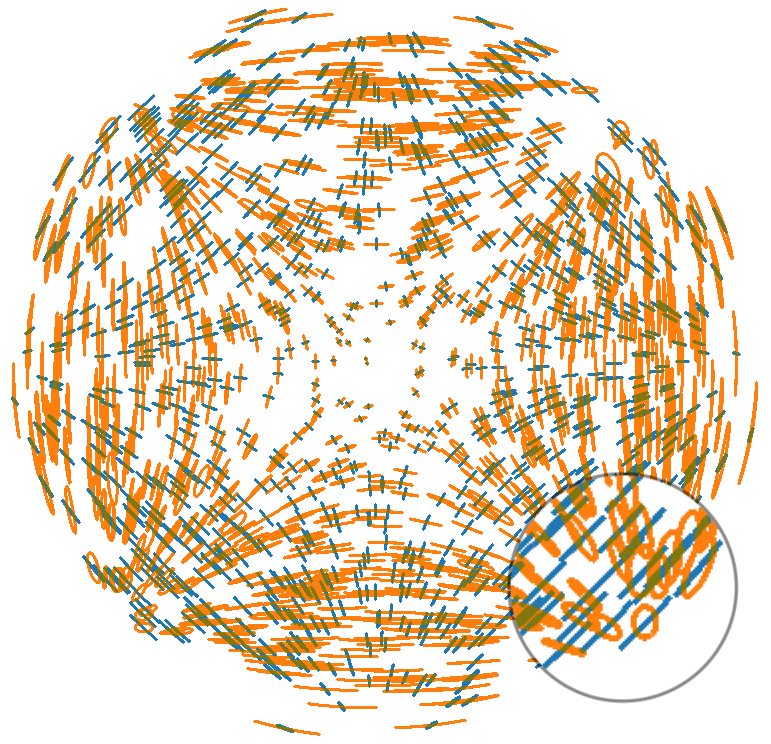
\includegraphics[width=1.0\textwidth]{Chapter4/Figs/Raster/fullstar.png}
\caption{\label{fig:ccc} The orthographic projection of a simulated set of $1000$ stars, as observed from the Earth looking in the negative $z$ direction. With a monochromatic transverse-traceless gravitational wave travelling down the $z$-axis, the apparent positions of the stars are plotted over a whole gravitational wave time period. This plot uses \cref{eq:nff} and does not take the liberty of a far-field limit assumption. Note the magnified area highlighting the elliptical shapes of the apparent oscillating star paths. The blue star paths--corresponding to the $+$-polarised gravitational wave resulting in--are also elliptical, however their width is far smaller and harder to observe. This is due to loss of generality stemming from the photon travelling from negative $z$ to positive $z$, meanwhile the gravitational wave travels from positive to negative $z$. Note, the $xy$-plane parallel with the page and the orientation is such that the horizontal is the $x$-axis and vertical is $y$-axis.}
\end{figure}



\section{Further Work and Conclusions}


From \Cref{ch:chapter3} that control variate subsampling should result in significantly more accurate nested sampling calculations than the Voronoi subsampling method used by Ref \cite{Mihaylov_2020} for general likelihoods that use subsampling. However we also find that, for this specific problem of astrometric deflection analysis, control variate subsampling shows task-specific advantages. Control variate subsampling will be better at dealing with more detailed gravitational wave astrometric deflections, even accounting for the star term causing the ellipse. The `star term' is the effect the gravitational wave has upon the photon as it is emitted from the star. The far-field equations we used earlier had this ignored and only accounted for the Earth term. The Earth term being the gravitational wave's interaction with the star photon upon measurement at the Earth. This will allow for much more accurate gravitational wave detections along with precise parameter estimations. An intuitive way to think of why Voronoi averaging does not bode well with varying astrometric deflection directions within a Voronoi cell is: imagine two stars with completely opposite astrometric deflections within one Voronoi cell, if they are both averaged over, then both deflections cancel out and we measure no signal at all for the gravitational wave. When it comes to the parallel astrometric deflections condition (ii) and using the full expression without approximations, not even a singular star itself would have a straight path for its astrometric deflection; thus the parallel astrometric deflections requirement becomes highly unlikely to be fulfilled.

Control variate subsampling could also be of use in determining the Bayesian evidence, $Z$, significantly more accurately than Voronoi subsampling. This would in turn be used for model comparisons and normalising the posterior distribution. We shall follow up this work with an explicit calculation of the results in \cite{Mihaylov_2020} using both Voronoi and control variate methods to do a side by side comparison. We plan on explicitly doing the control variate assisted Bayesian analysis suggested in this chapter. 

%!TEX root = ../thesis.tex
%*******************************************************************************
%****************************** Third Chapter **********************************
%*******************************************************************************
\chapter{Conclusions and further work}\label{ch:chapter5}

% **************************** Define Graphics Path **************************
\ifpdf
    \graphicspath{{Chapter5/Figs/Raster/}{Chapter5/Figs/PDF/}{Chapter5/Figs/}}
\else
    \graphicspath{{Chapter5/Figs/Vector/}{Chapter5/Figs/}}
\fi

\section{Conclusions}

In \cref{sec:limitations} we listed two of the most fundamental limitations on nested sampling: the accuracy of Bayesian evidence calculations and the computational limit on the size of the datasets. The basis of this thesis was to propose methods to overcome these limitations. We found promising results in both methods proposed to tackle these problems. Gradient nested sampling showed preliminary promise in providing a fundamental increase in the core nested sampling algorithm. John Skilling himself predicted such improvements should be possible, given that a `prior on curves' should exist but needs to be found. Additionally, the control variate subsampling scheme we introduced in \cref{ch:chapter3} demonstrated the potential for substantially cutting computational costs over the widespread methods such as simple random sampling (SRS) and averaged-deterministic-subsampling. A further contribution of this thesis is a novel examination of the compatibility of non-deterministic likelihoods with nested sampling. Whilst these are only preliminary results, they provide a promising avenue for future MPhil \& PhD projects. 

\section{Related Work; Big Data, Machine Learning, and Cosmology}

\subsection{Stochastic Gradient Descent}


The most extensively employed optimization algorithm in modern machine learning is stochastic gradient descent (SGD). The work on efficient subsampling discussed in \cref{ch:chapter3} is directly applicable to SGD.

SGD involves sampling a subset of the available dataset to approximate the true gradient. The reason for subsampling is computational restrictions. As further work, we are looking to apply the control variate subsampling method introduced in \cref{ch:chapter3} to improve the efficiency of SGD. Another takeaway from \cref{ch:chapter3} that may be analogously applied to SGD is that non-deterministic subsampling is significantly superior to deterministic subsampling in most cases (due to large number of samples cancelling out the biases), so SGD should always utilise non-deterministic subsampling (i.e.\ sample a different subset at each sampling iteration). However, this non-determinism may cause several complications with convergence as we will discover in \cref{ch:chapter3} as well.


In \cref{ch:chapter2} we utilise a concept analogous to SGD: in our proposed `gradient nested sampling', we use the stochastically-determined gradient of the likelihood function to guide our choice of the prior volume estimate. A takeaway from \cref{ch:chapter2} that may be analogously applied to SGD is that we found that it is helpful to do a rolling sum of the stochastic gradient over a local region to get a better estimate. This rolling average could be utilised in a SGD algorithm as well.

\subsection{Bayesian Neural Networks Incorporating Nested Sampling.}


In Ref~\cite{https://doi.org/10.48550/arxiv.2205.11151} David Yallup, Will Handley et al. apply nested sampling to Bayesian Neural Networks. Further work on this MPhil thesis lay in the realms of applying \cref{ch:chapter2}'s gradient nested sampling to BNNs and utilising \cref{ch:chapter3}'s efficient subsampling in the BNN training.


\subsection{Batch/Offline and Online Learning}

Batch/offline learning is a form of deterministic subsampling of data-space. Data accumulated over a certain period of time is used to train a model. For example, data could be updated weekly. The issue with batch learning is that it is costly to retrain data. Whenever the data is updated by the new batch the whole parameter landscape, on which the neural network performs gradient descent is perturbed. This means that much of the previous training is nullified and the NN must thus be retrained. However, this means that the training is done on chunks of deterministic datasets and the datasets are altered in intervals. However, with online learning, the data is updated incrementally in real time. This means that for the duration of the online training, the data is non-deterministic. In \cref{ch:chapter3}, we go in-depth into the pitfalls of deterministic subsampling of data space and how it can be inferior to non-deterministic subsampling. Some of the lessons we learnt could be analogously applied to offline/online learning. For example in relation to dealing with convergence issues related to non-deterministic data and how it could be superior to use online learning--analogously to how non-deterministic subsampling subsampling is shown to be superior in \cref{ch:chapter3}.


\subsection{Further Cosmology Work}
More further work lies in the realms of carrying out a similar Bayesian analysis for measuring redshift, as is outlined for the astrometric deflections in \cref{ch:chapter4}. This is another similar method to extract gravitational waves using star photon measurements. It can be performed by utilising the frequency perturbations of the measured photons. This is mostly accomplished by analysing pulsar timing array datasets like NanoGrav~\cite{McLaughlin_2013}. We did not cover it in this thesis but will quickly go over it since our proposed control variate method would be of relevance in improving pulsar timing array~\cite{ 1975GReGr...6..439E} data analysis accuracy. The redshift would be observed as~\cite{Mihaylov_2020}
%
\begin{equation}
z=\frac{(n^{i} n^{j})}{2(1-\textbf{q} \cdot \textbf{n})}[h_{ij}(E)-h_ij(S)],
\end{equation}
%
This result was derived in Ref~\cite{Mihaylov_2020} using Ref~\cite{KAUFMANN1970}. This can be thought of as an analogous equation to \cref{eq:px,eq:py}. 

Beyond the above considerations, there are potentially endless applications within cosmology of the work done in this thesis. Many analyses in cosmology that utilise Bayesian inference could make use of efficient subsampling and gradient nested sampling's more accurate evidence computation. Whilst the results in this thesis are theoretical and preliminary, and thus require further development, they provide a useful starting point for future research.

%\include{Chapter6/chapter6}
%\include{Chapter7/chapter7}



% ********************************** Back Matter *******************************
% Backmatter should be commented out, if you are using appendices after References
%\backmatter

% ********************************** Bibliography ******************************
\begin{spacing}{0.9}

% To use the conventional natbib style referencing
% Bibliography style previews: http://nodonn.tipido.net/bibstyle.php
% Reference styles: http://sites.stat.psu.edu/~surajit/present/bib.htm

%\bibliographystyle{apalike}
\bibliographystyle{unsrt} % Use for unsorted references  
%\bibliographystyle{plainnat} % use this to have URLs listed in References
\cleardoublepage
\bibliography{References/references} % Path to your References.bib file


% If you would like to use BibLaTeX for your references, pass `custombib' as
% an option in the document class. The location of 'reference.bib' should be
% specified in the preamble.tex file in the custombib section.
% Comment out the lines related to natbib above and uncomment the following line.

%\printbibliography[heading=bibintoc, title={References}]


\end{spacing}

% ********************************** Appendices ********************************

% *************************************** Index ********************************

\end{document}
